\chapter{Results}

After four months of development, the program remains unfinished. Several unforeseen difficulties were encountered during the process, which required significantly more time than initially expected. As a result, there are not only some features still pending implementation, but also several existing issues that need to be resolved. The most important of these are:

\begin{itemize}
	\item \textbf{GUI freeze:} Occasionally, the interface freezes when switching between pages in the analysis window. Debugging efforts have shown that the program continues to run in the background, but the graphical interface becomes completely unresponsive, leaving no option but to force quit and restart the program.
	
	\item \textbf{Output to System Glitch:} This is the main issue referred to several times in the Acoustic Correction chapter. It renders the Bypass and EQ modules nearly unusable in real-time situations, as it introduces a glitch effect in the Output to System signal. After conducting various tests, I concluded that the problem likely stems either from how data is managed within the DSP window or from how this window interacts with the output stream. The glitch appears to be caused by repeating or skipping certain data blocks in the output stream. When the program is configured with a very large block size, it becomes clearly audible that some blocks are played more than once, while others are skipped entirely.
\end{itemize}

Another minor issue is:

\begin{itemize}
		
	\item \textbf{Filter Algorithms:} It would be beneficial to invest more time into researching and designing better filters in order to achieve more accurate and appropriate results, both for analysis and correction purposes.
	
	\item \textbf{User Limitations:} Additionally, the graphical user interface (GUI) could be more intuitive and requires refinement to offer clearer options and a better representation of ongoing processes. Furthermore, it is necessary to implement more constraints to prevent misconfigurations or malfunctions. For example, since the program uses the Sounddevice library and handles both inputs through a single input stream, both channels must originate from the same sound card. However, the current version of the program still allows users to select different sound cards for each input channel—an option that should be restricted to avoid improper operation.
	
\end{itemize}

But not all news is bad. As will be shown in the \textbf{Final Test} section below, the program is already partially usable, and the developed tools work quite well.

\section{Final tests}

For the final test, which involved a real-world scenario, I had the privilege of accessing professional equipment and a real theater. The venue was the \textbf{Teatre del Coro}, located in Sentmenat, Spain, and managed by the non-profit cultural association \textit{Societat Coral Obrera la Gloria Sentmenatenca}. The equipment available for the test was:

\begin{itemize}
	\item \textbf{EVO 4:} External USB audio interface, used as the sound card for the program.
	\item \textbf{Audix TM1:} Measurement microphone, used as the source for the \textbf{Input from System} signal.
	\item \textbf{Mackie SRM-750:} Loudspeaker, responsible for playing the \textbf{Output to System} signal.
	\item \textbf{External Laptop:} Device used to generate the \textbf{External Input} signal.
	\item \textbf{Behringer X32 Compact:} The theater's digital mixing console. It is required to route signals to the speaker. Since it is part of the system, it will also be used to compare the analysis tools of the RTA+C program with the built-in tools of the mixer.
\end{itemize}

The sound card and the measurement microphone were kindly provided by \textit{IMESDE, Integració, Distribució i Enginyeria Escènica, S.L.}, a private company located in La Garriga, Spain. All the devices used can be seen in Figure~\ref{fig:Coro_setup}.

The first step was to place the measurement microphone. It was important to choose a good position where the microphone could capture the sound from a single representative point in the room. The first parameter to define was the microphone height. This venue is very versatile throughout the week, and the seats can be removed. However, events held without the seats typically do not require the use of the theater's sound system. Therefore, it was more appropriate to take measurements with the seats in place. Unfortunately, on the day I was able to perform the measurements, the seats had been partially removed. Nevertheless, I positioned the microphone at the average height of a seated person, as shown in Figure~\ref{fig:Mic_pos1} and Figure~\ref{fig:Mic_pos2}.

\begin{figure}[H]
	\centering
	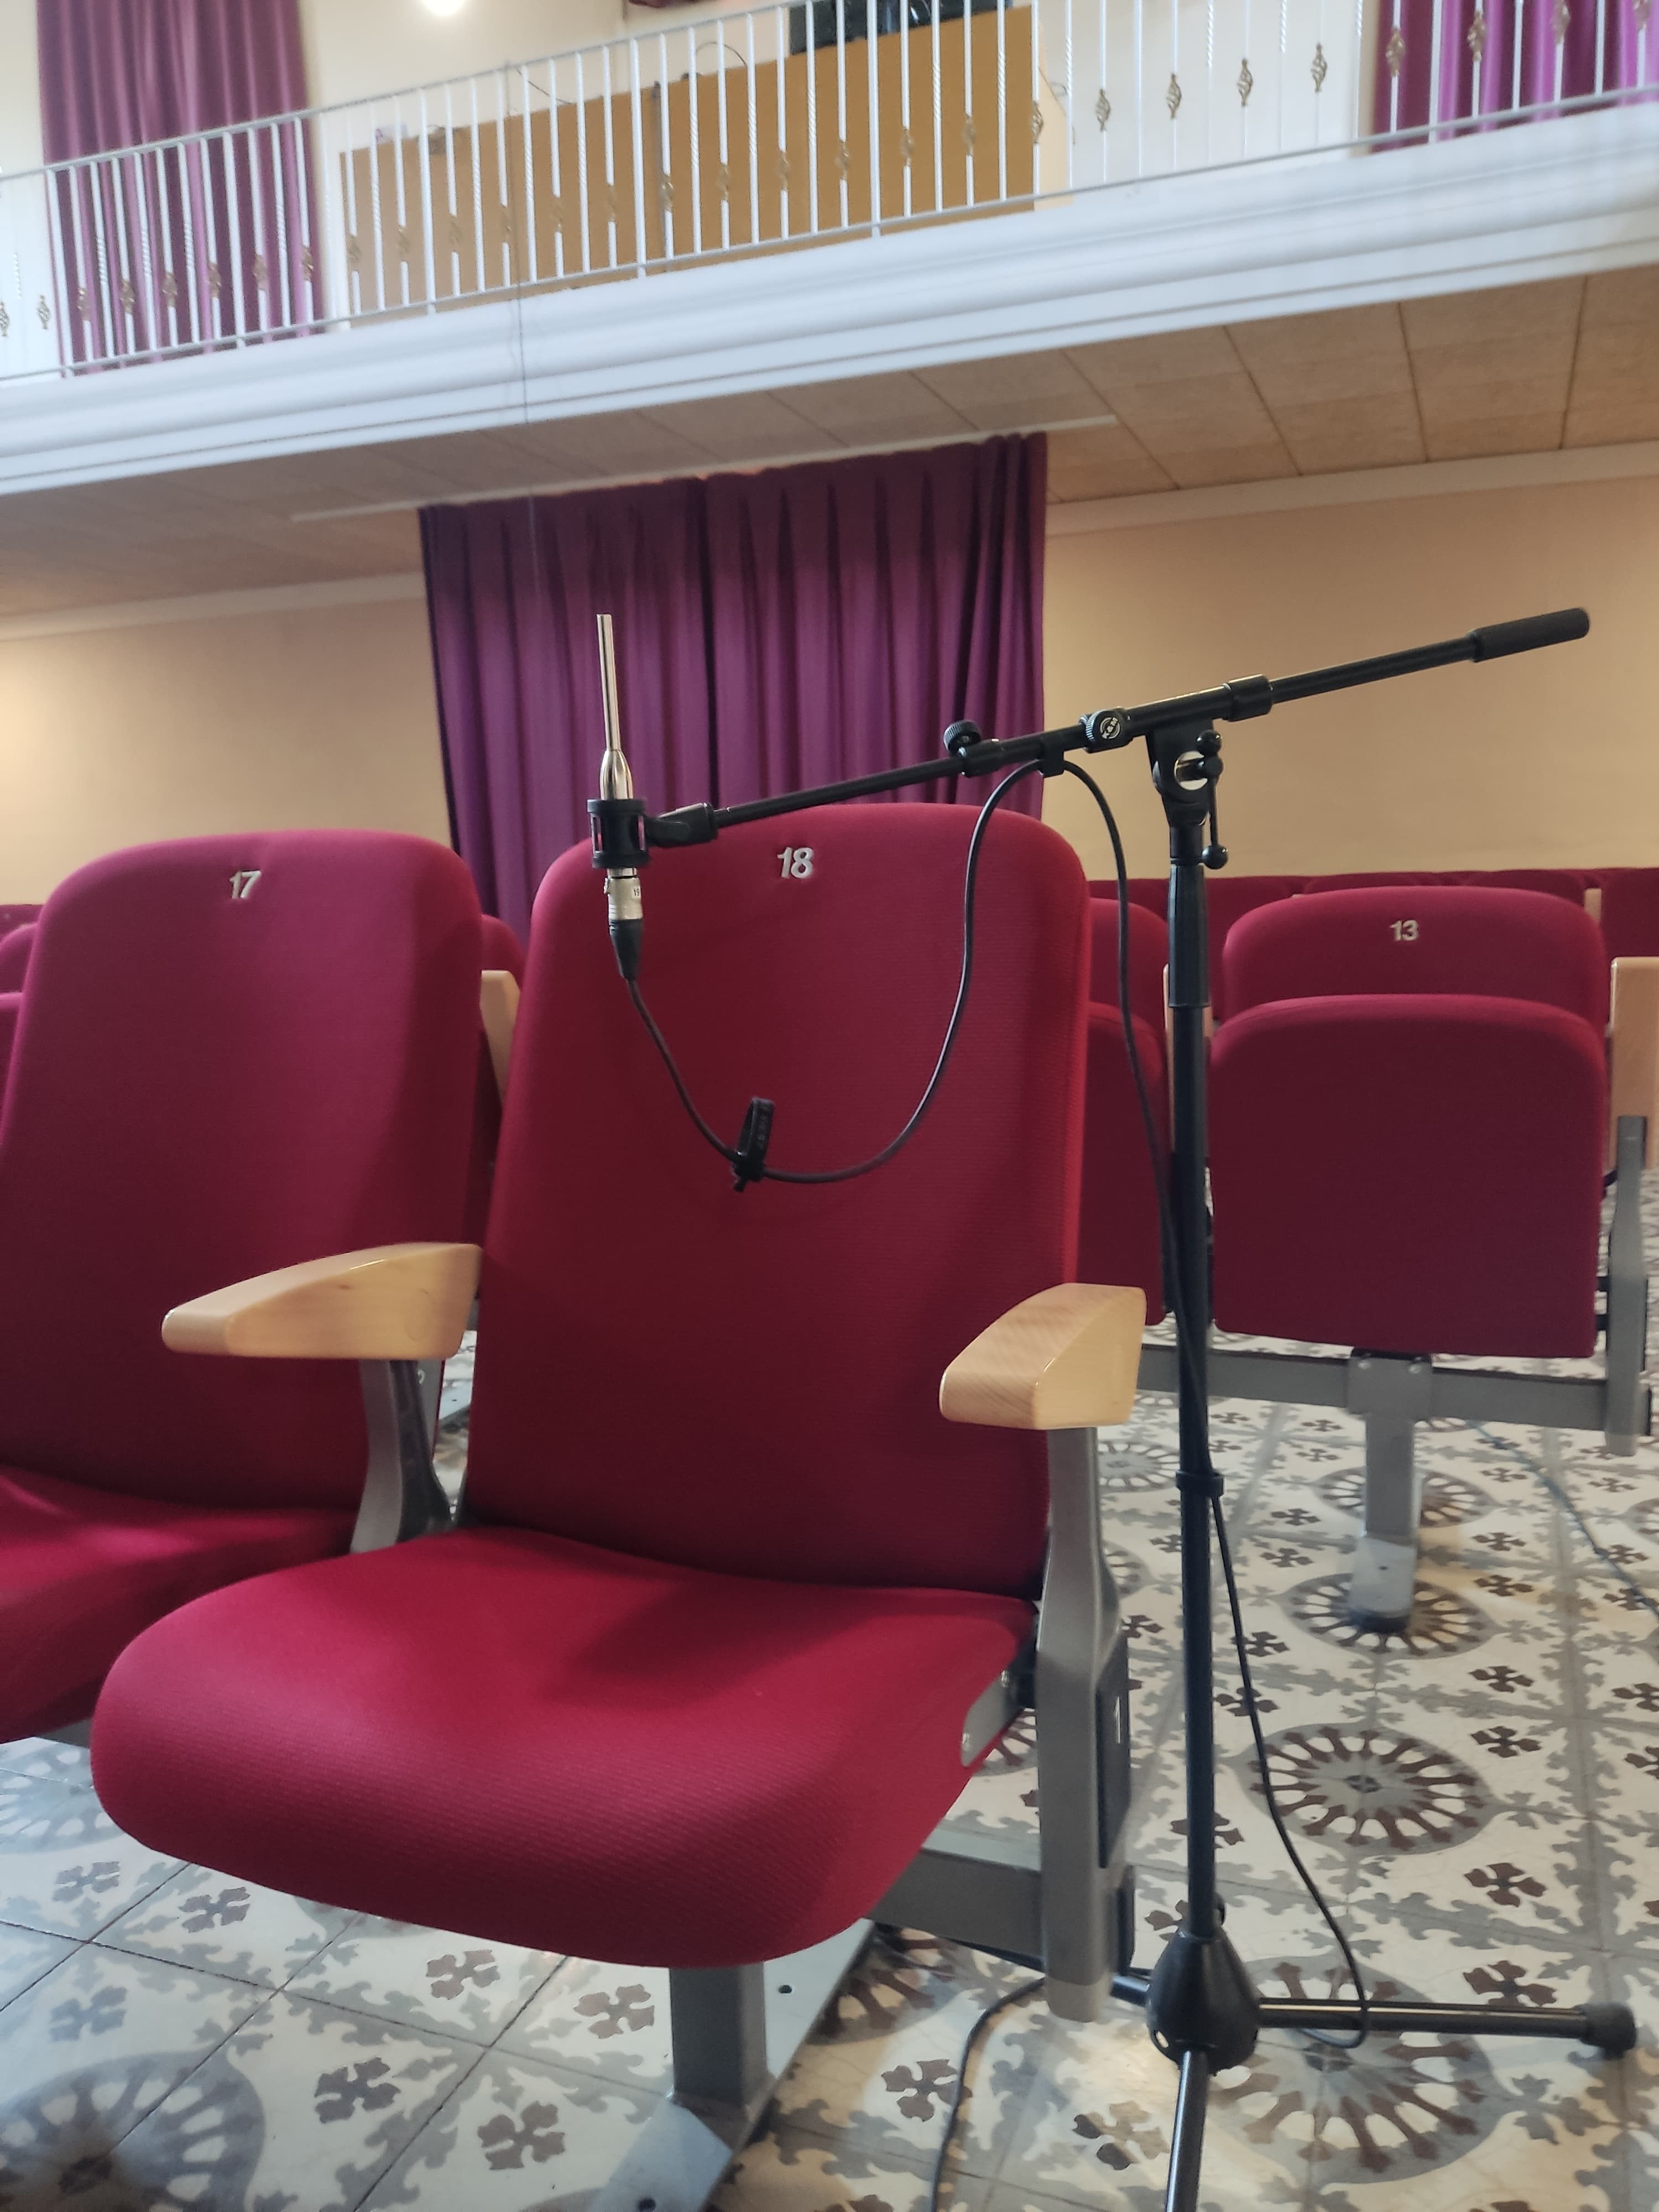
\includegraphics[width=0.6
	\linewidth]{Figures/Coro_micpos1.jpeg}
	\caption{Microphone height relative to the seat}
	\label{fig:Mic_pos1}
\end{figure}

\begin{figure}[H]
	\centering
	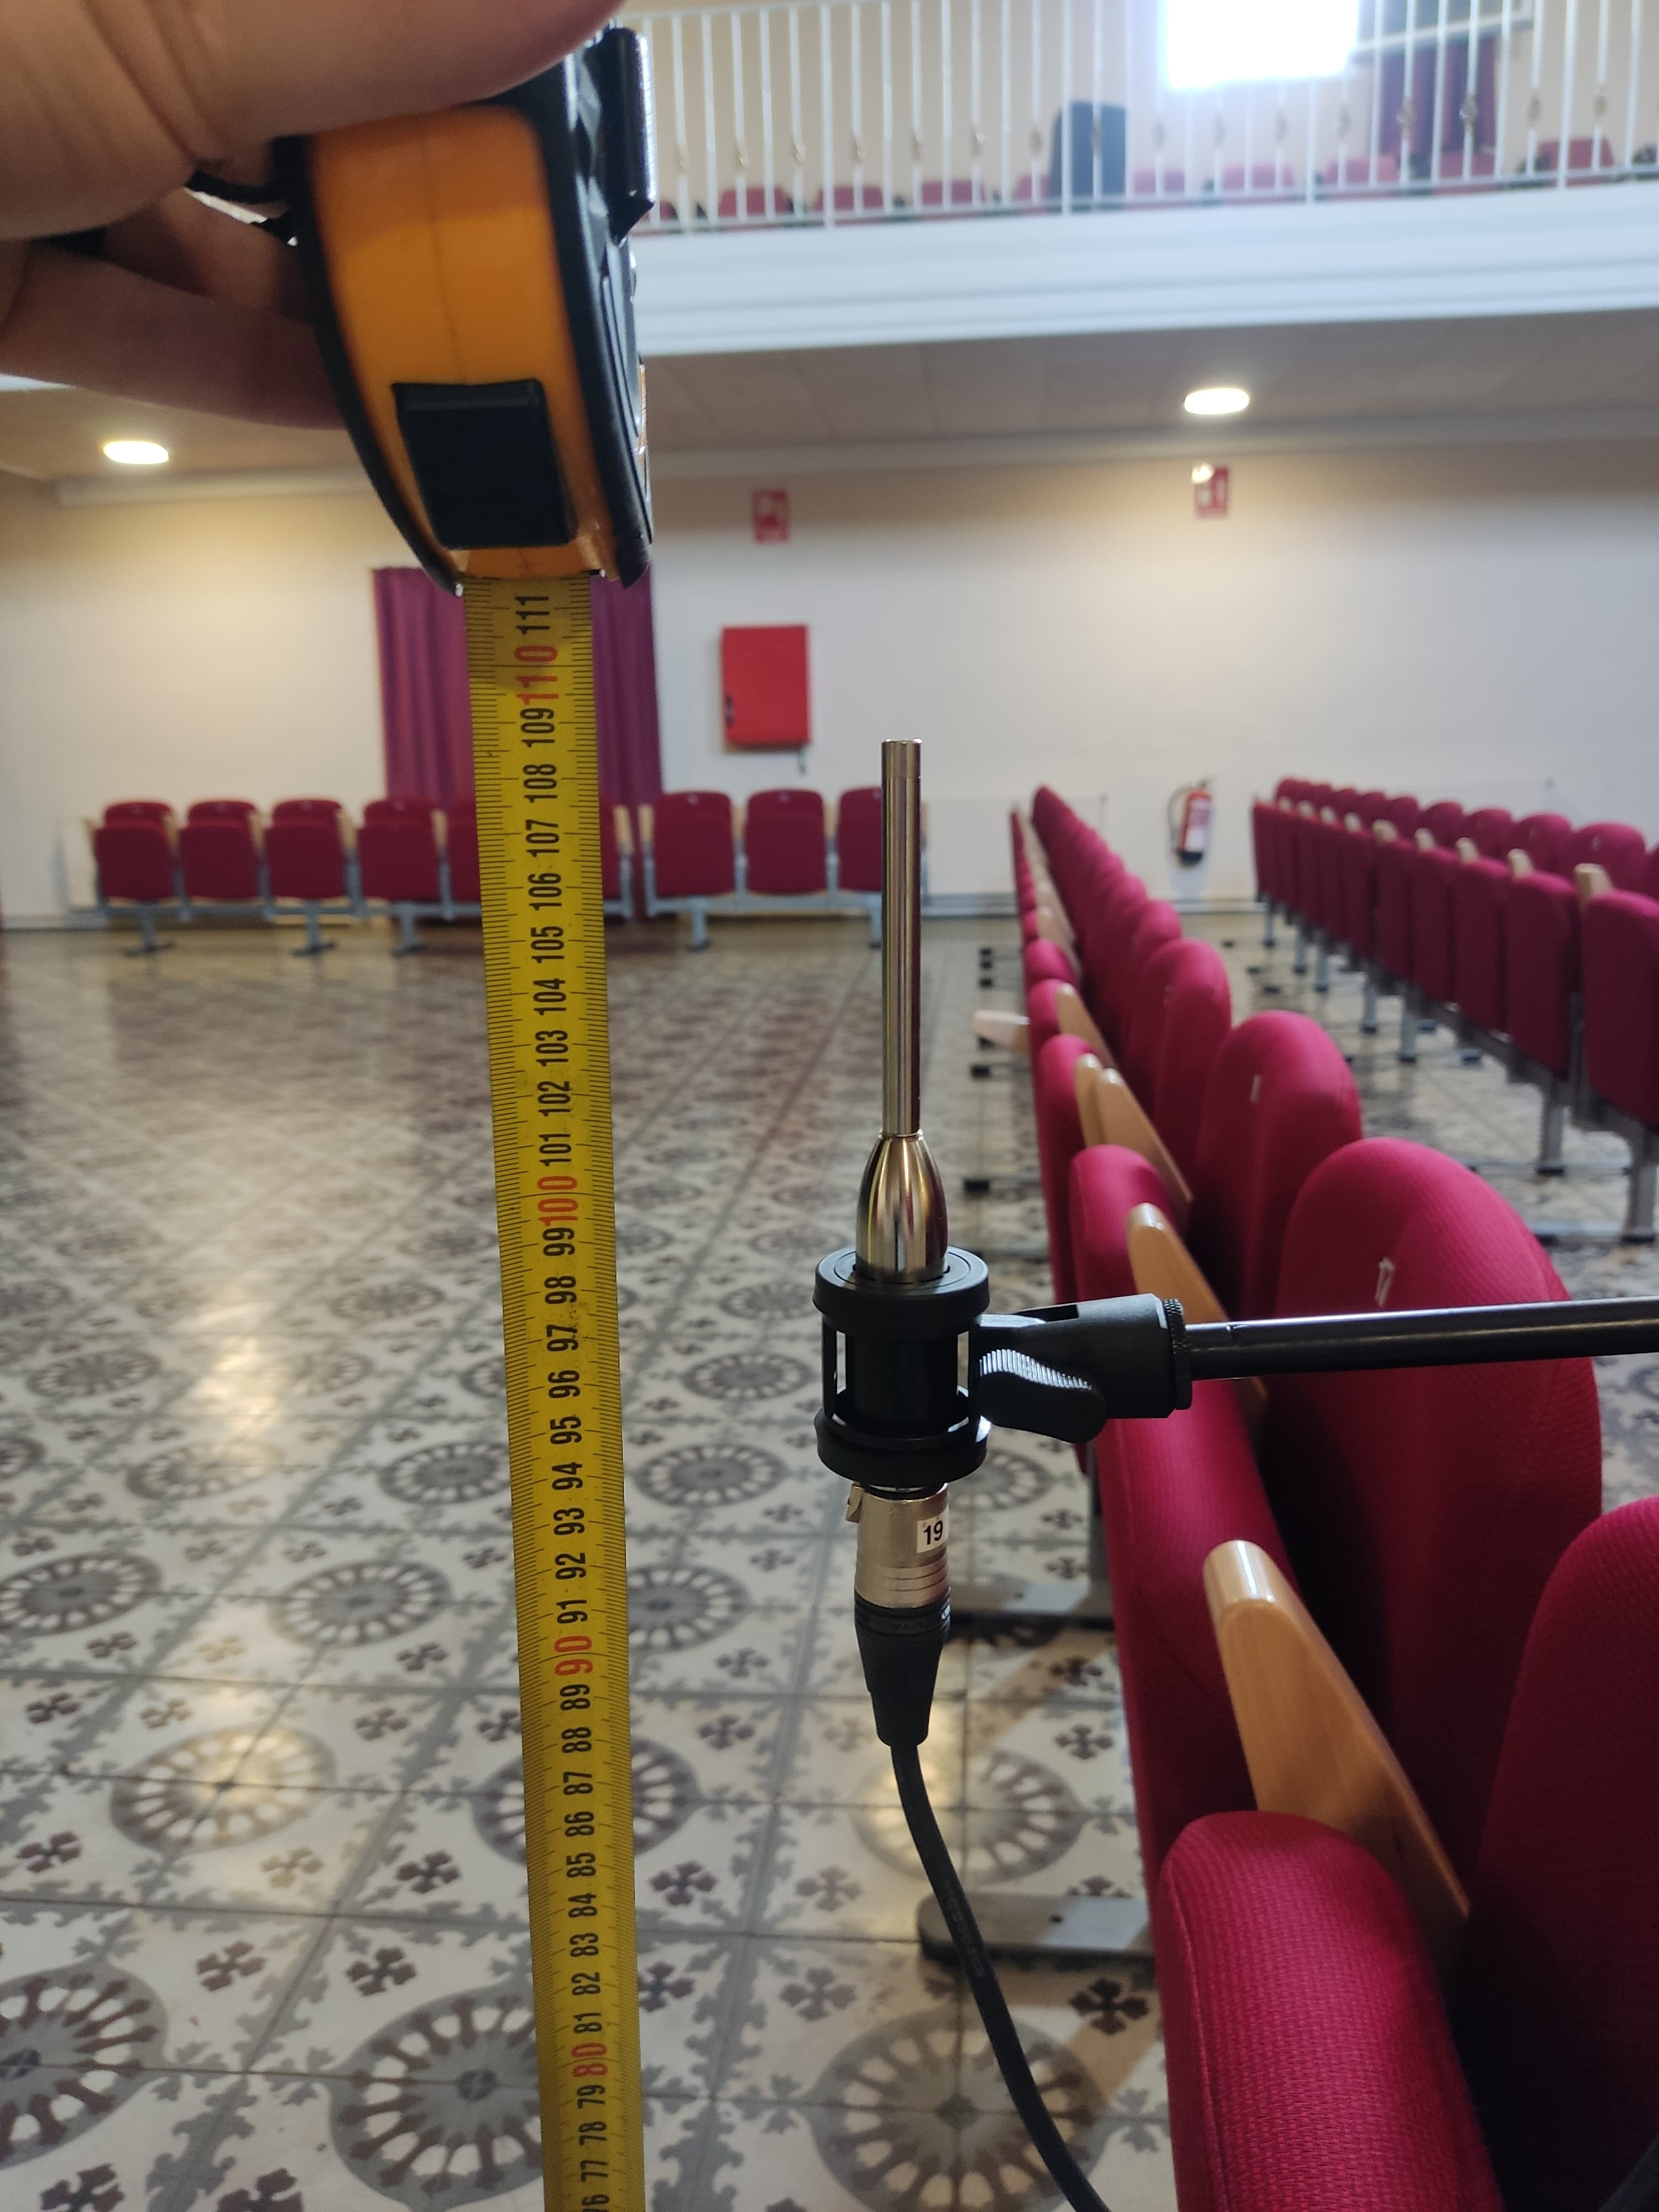
\includegraphics[width=0.8
	\linewidth]{Figures/Coro_micpos2.jpeg}
	\caption{Microphone height = 1.1m}
	\label{fig:Mic_pos2}
\end{figure}

Next, the microphone had to be placed at a representative point in the room. Since I was measuring only one speaker and the program operates in mono, the position had to be one where the speaker had good coverage and where the microphone was as close as possible to the center of the audience area. I decided to place the microphone approximately halfway through the depth of the room. Starting from a position where the speaker was directly in front of the microphone, I shifted it slightly to the right to bring it closer to the actual center of the room. As shown on figure~\ref{fig:Mic_pos3} and figure~\ref{fig:Floor_section}.
\begin{figure}[H]
	\centering
	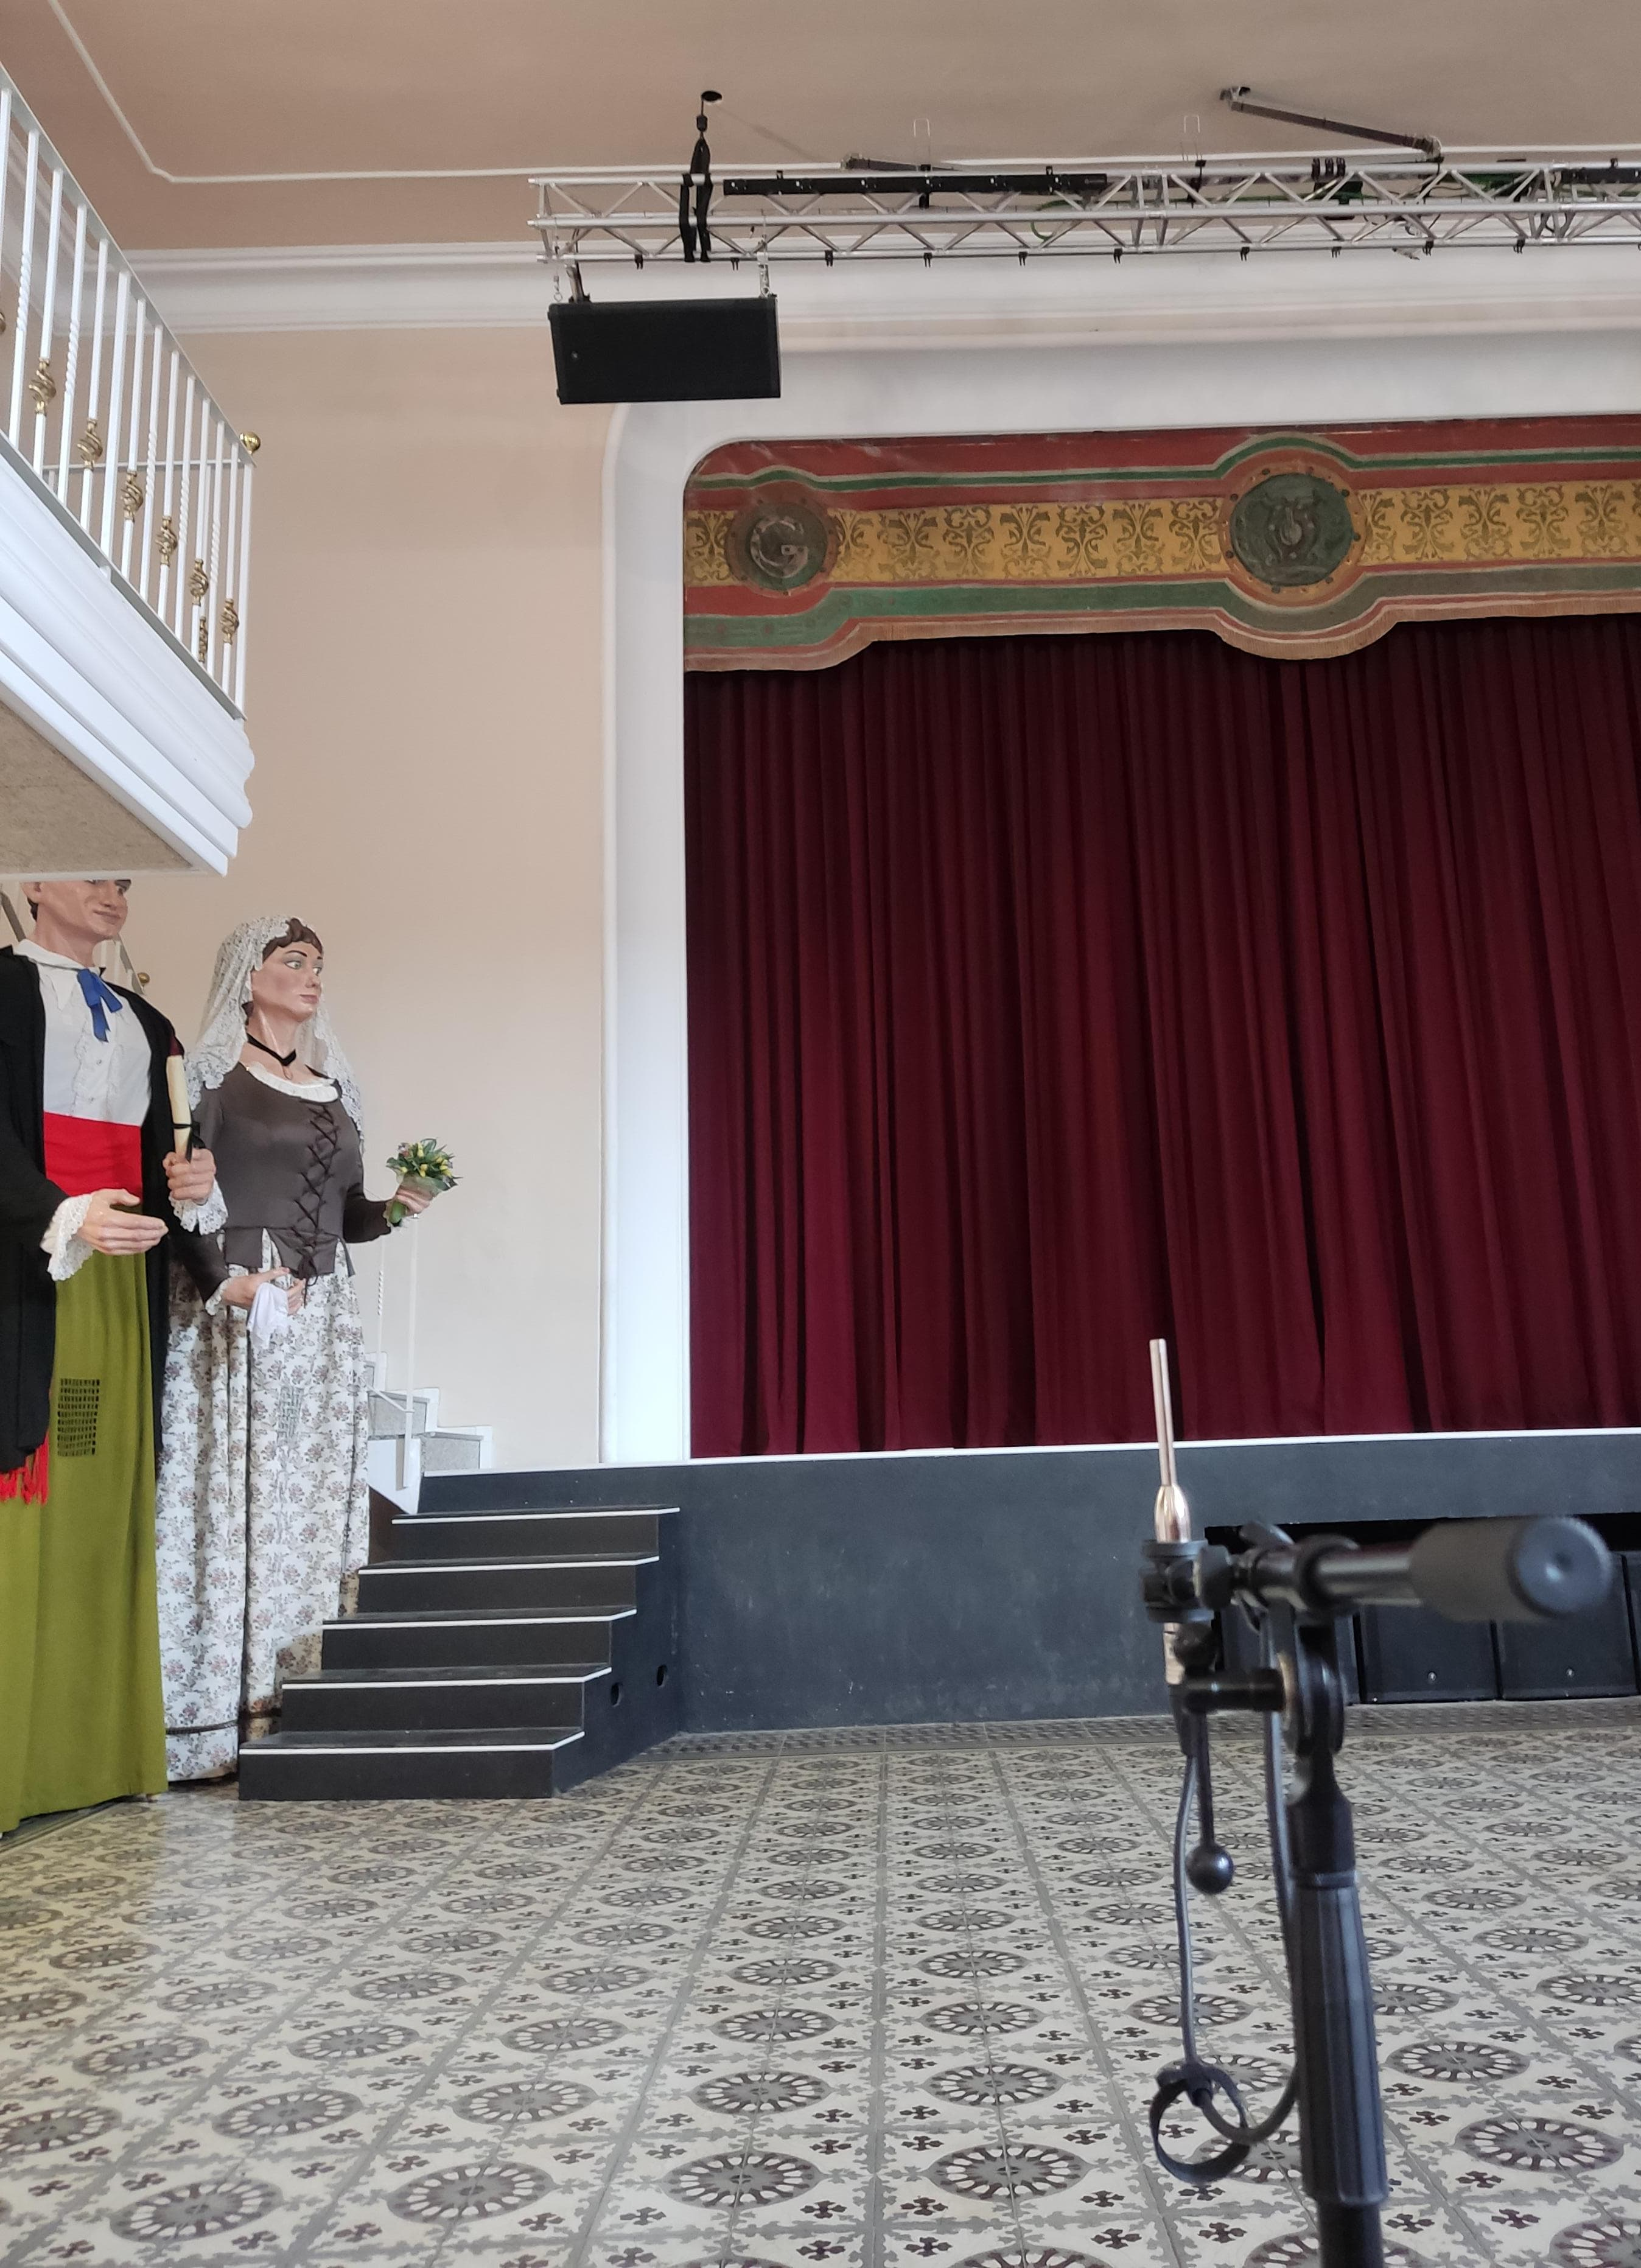
\includegraphics[width=0.8
	\linewidth]{Figures/Coro_micpos3.jpeg}
	\caption{Microphone position relative to the speaker}
	\label{fig:Mic_pos3}
\end{figure}

\begin{figure}[H]
	\centering
	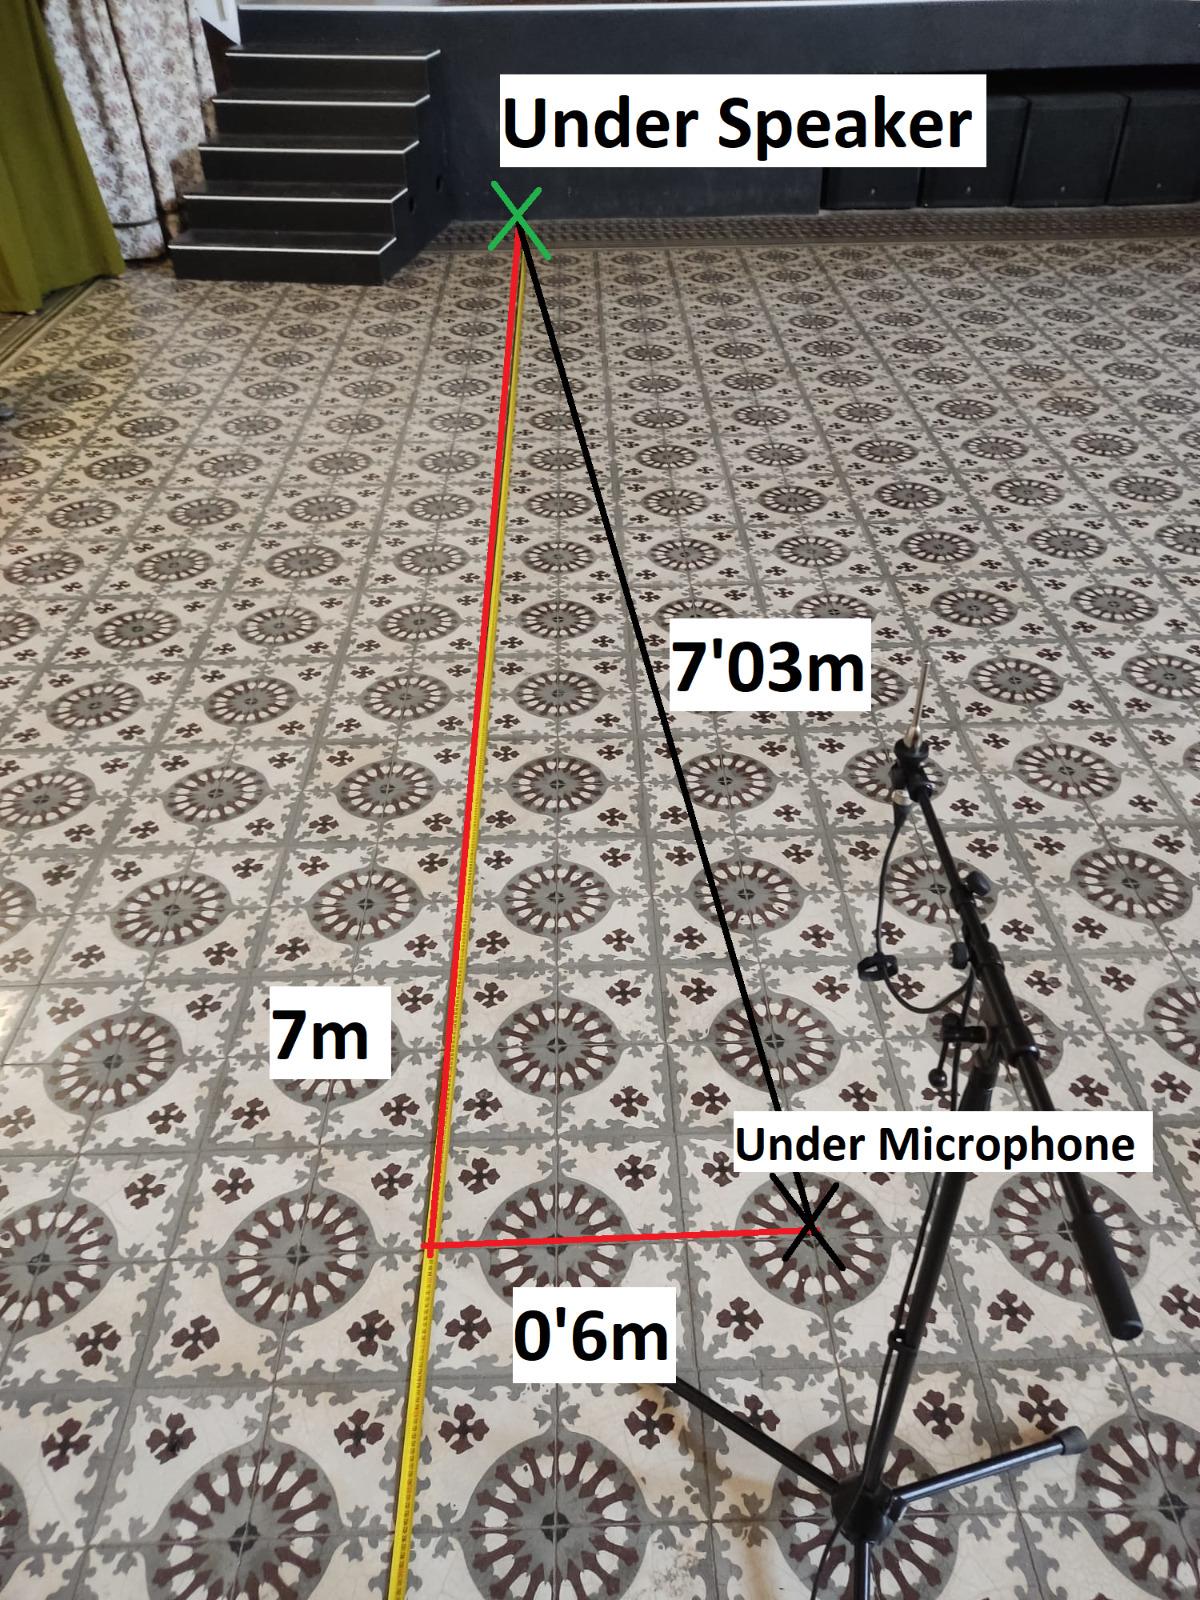
\includegraphics[width=0.8
	\linewidth]{Figures/Coro_floor_trigo.jpeg}
	\caption{Horizontal distance between speaker and microphone}
	\label{fig:Floor_section}
\end{figure}

Knowing that the speaker is suspended from a rigging bar at a hieght of approximately 6.5 m, and substrating the microphone height, the vertical distance between the two is around 5.4 m. Additionally, the horizontal distance—shown in Figure~\ref{fig:Floor_section}—is 7.03 m. Using basic trigonometric calculations, we can determine that the total distance between the speaker and the microphone is approximately 8.86 m, as illustrated in Figure~\ref{fig:spk-mic}.


\begin{figure}[H]
	\centering
	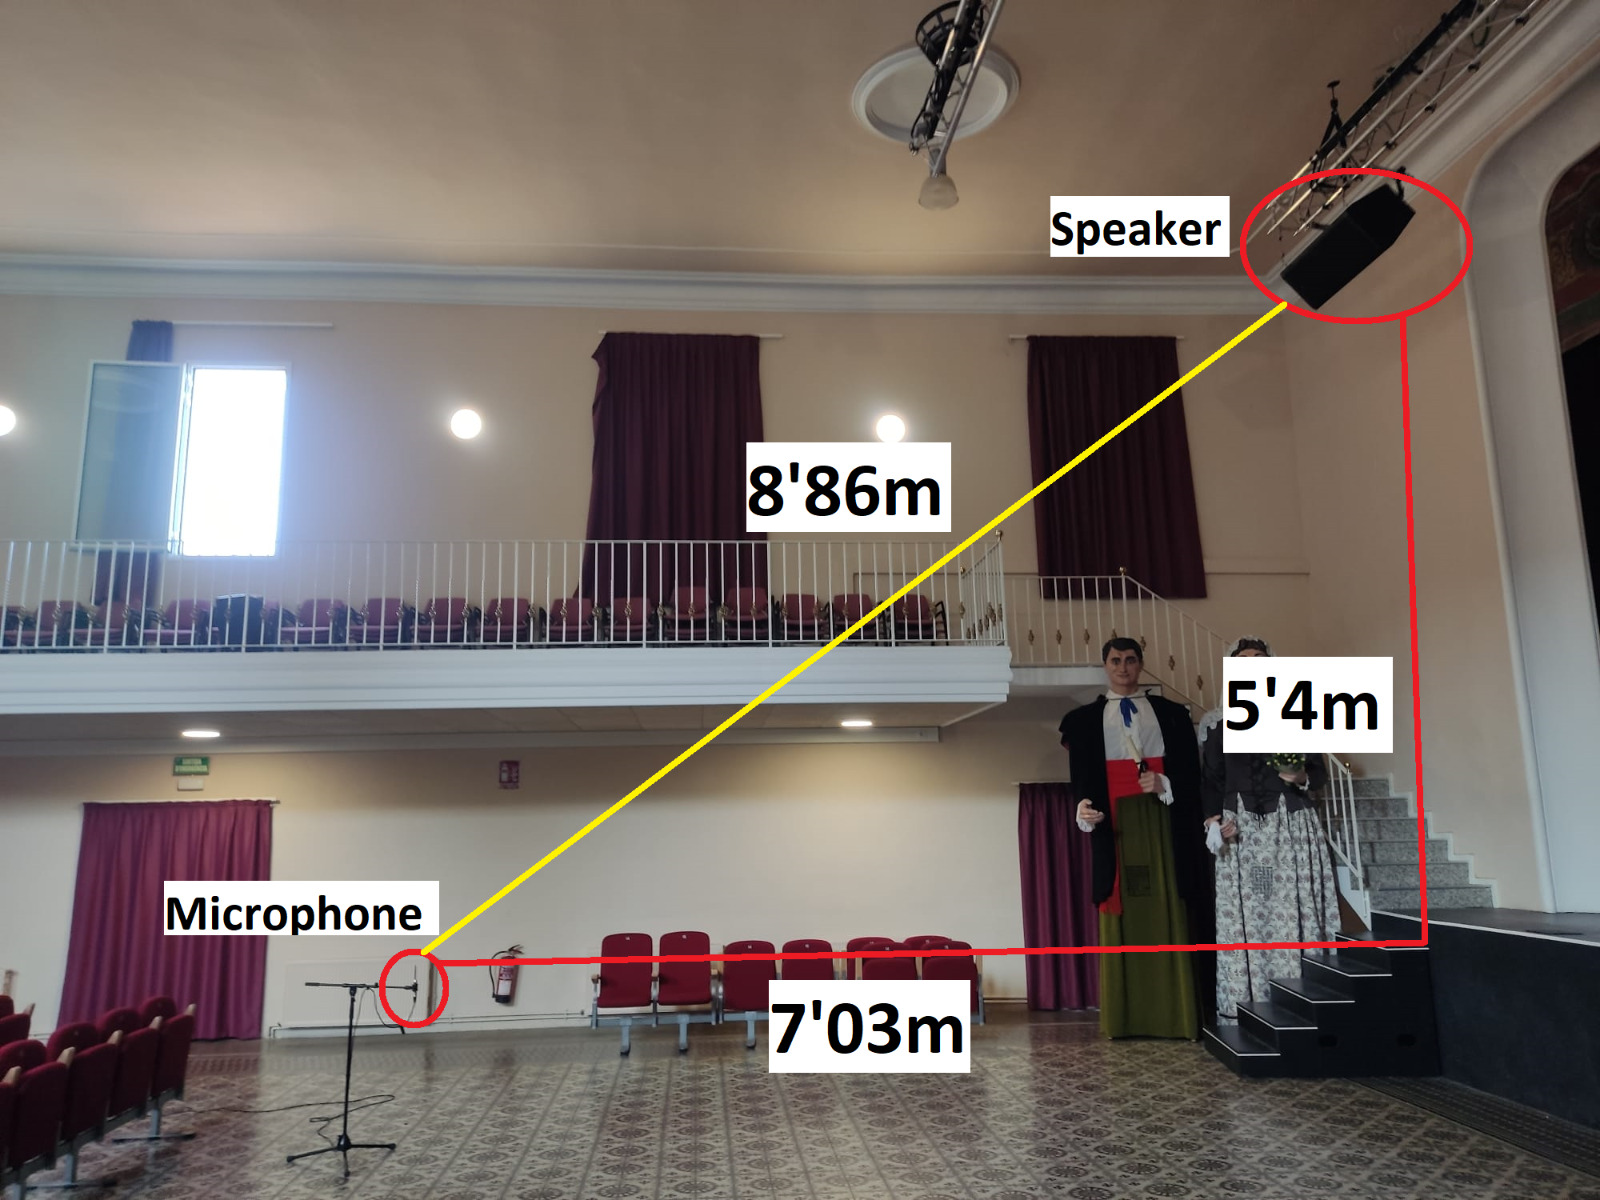
\includegraphics[width=0.8
	\linewidth]{Figures/Coro_section_trigo.jpeg}
	\caption{Distance between microphone and speaker}
	\label{fig:spk-mic}
\end{figure}

Once the microphone was positioned, it was time to set up the rest of the equipment, as shown in Figure~\ref{fig:Coro_setup}.

\begin{figure}[H]
	\centering
	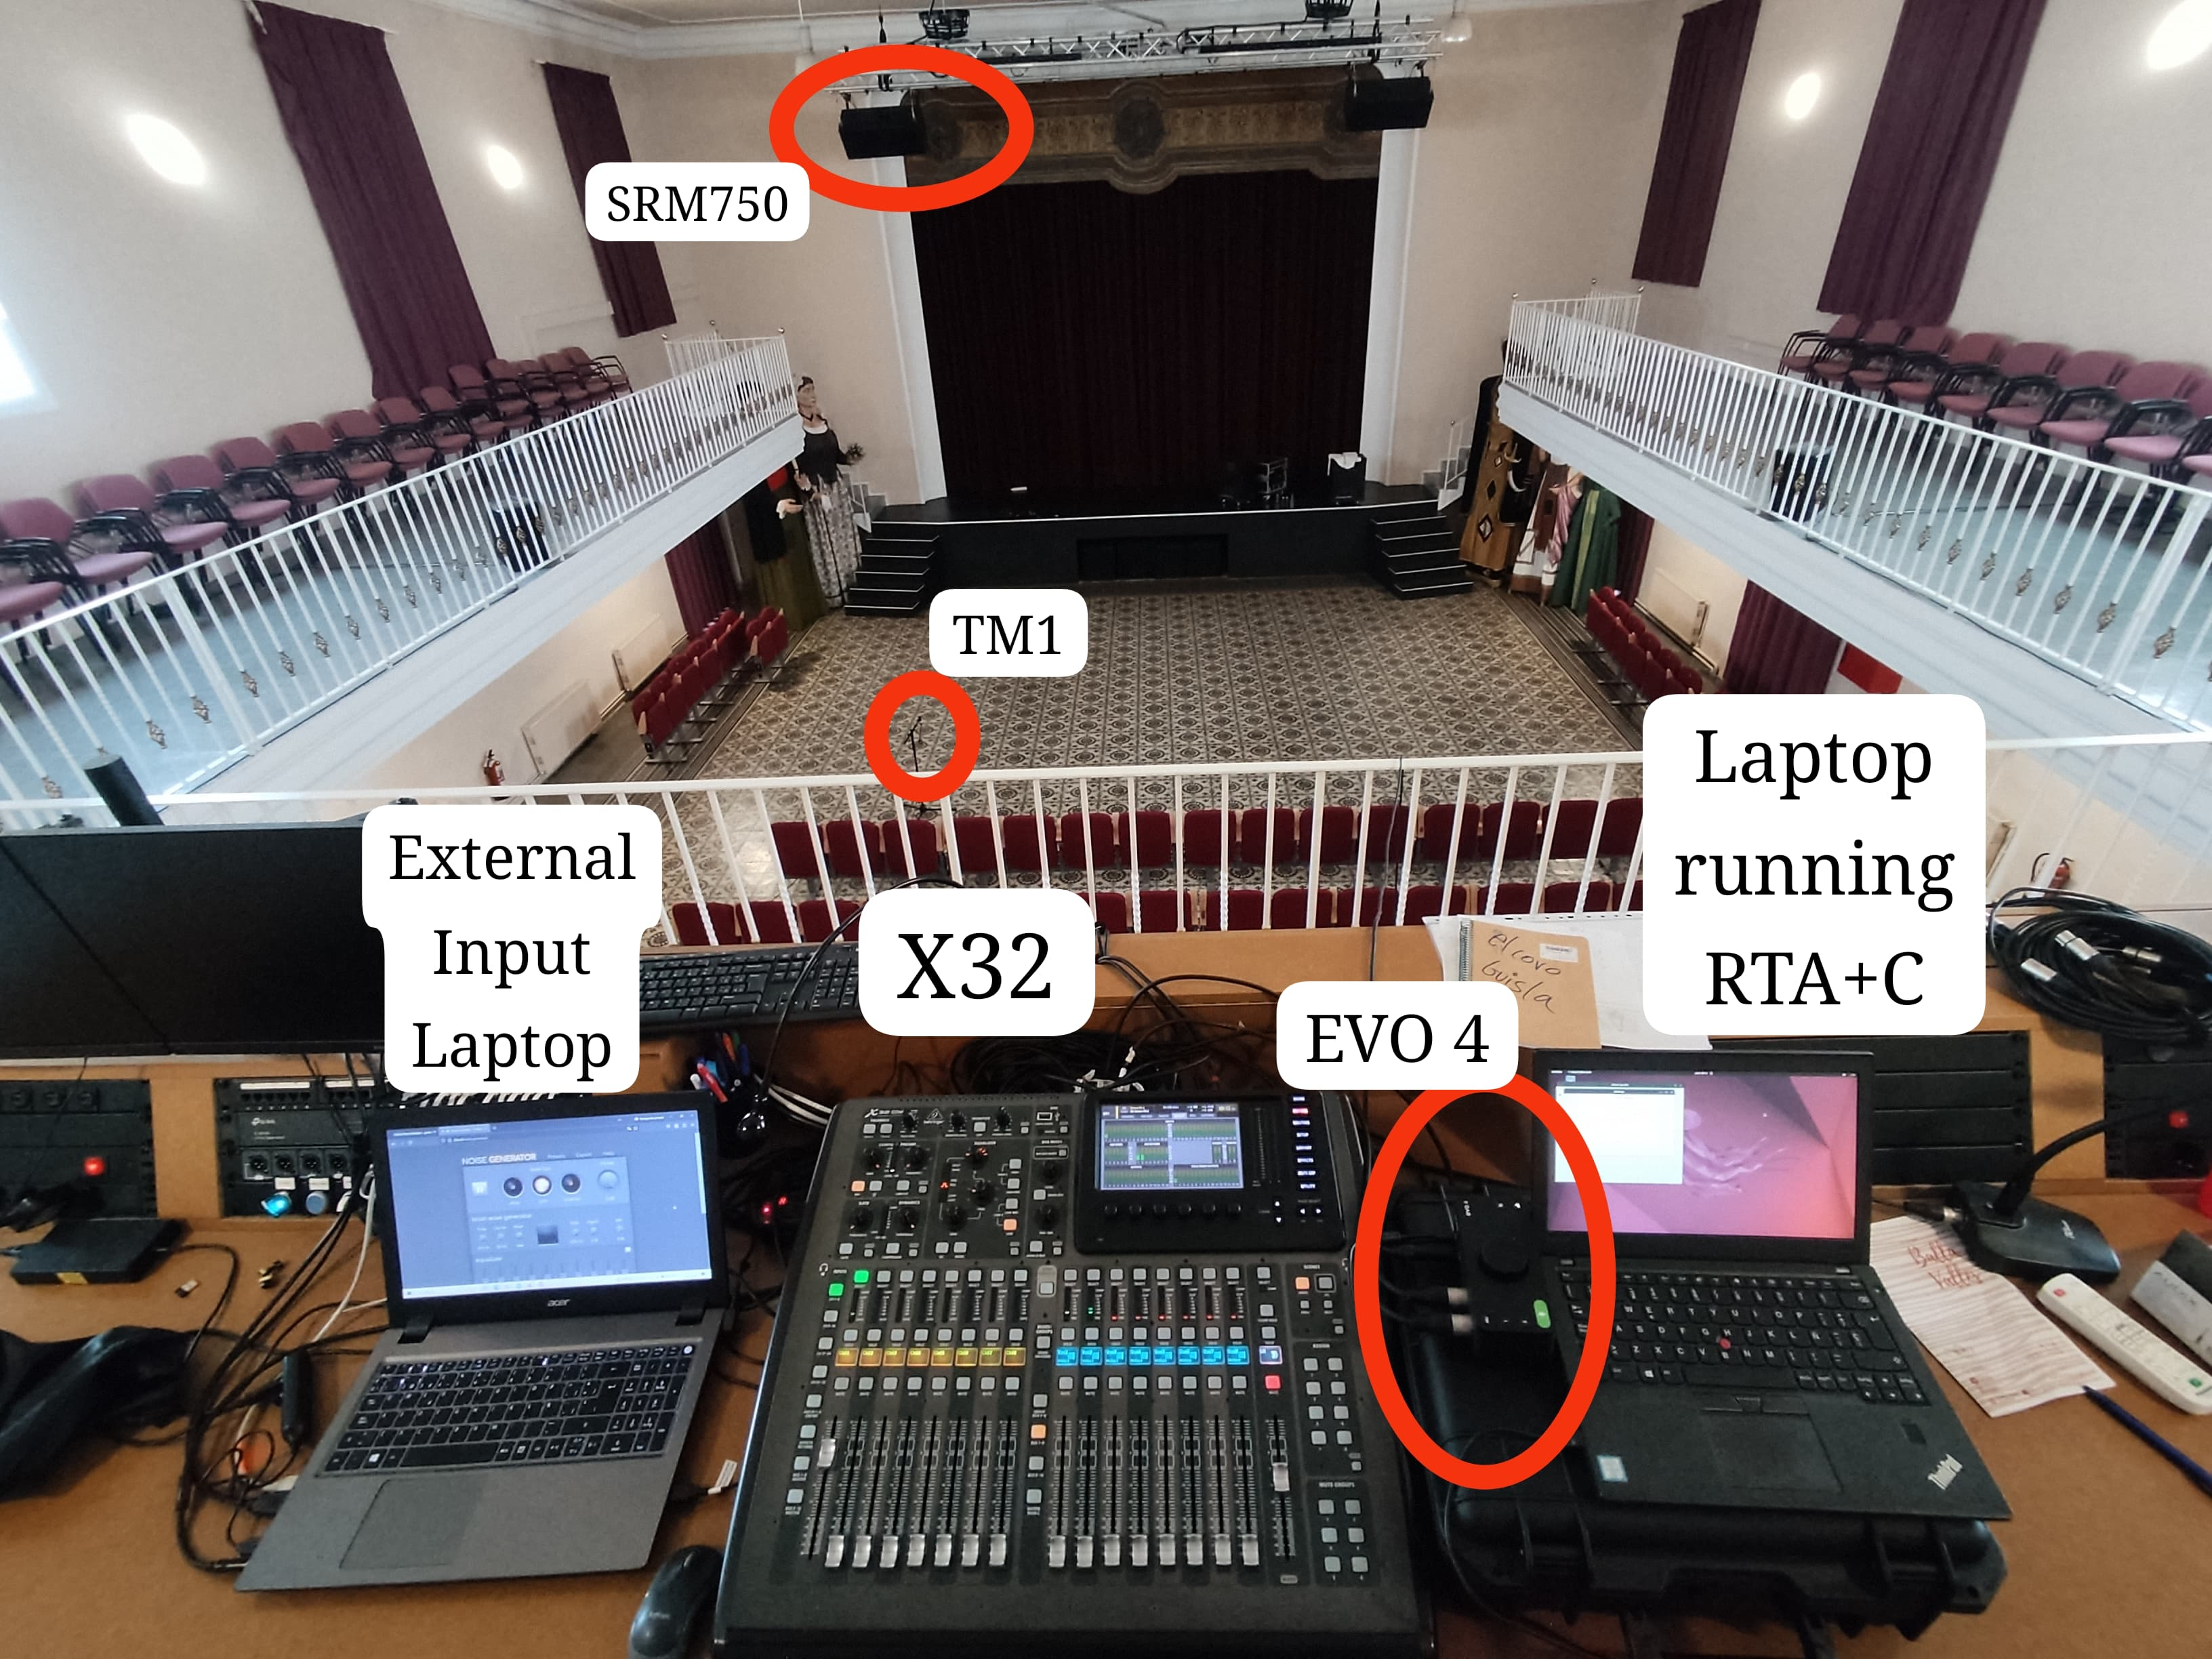
\includegraphics[width=0.8
	\linewidth]{Figures/Coro_setup.jpeg}
	\caption{All equipment set up}
	\label{fig:Coro_setup}
\end{figure}

In order to enable comparison between our software solution and the built-in tools of the digital mixing console (\textit{X32}), all signals must be routed through the \textit{X32}, as it offers advanced routing and distribution capabilities. Additionally, the console must be properly configured to route the signals correctly. Remember that we are using the \textit{EVO 4} as the audio interface for the RTA+C software, as shown in the following connection diagram.

\begin{figure}[H]
	\begin{center}
		\vspace{-2mm}
		\tikzsetnextfilename{connectio_setup}
		\begin{tikzpicture}[node distance=30mm,on grid,auto, scale=1, bend angle=45]
			
			every node/.style={font=\small};
			
			\node (q_ext) [draw, rectangle, minimum size=1cm] {Laptop (source of sound)};
			\node (q_X32_ext) [draw, rectangle, minimum size=1cm, right=of q_ext, xshift=2cm]{X32 - External Input};
			\node (q_evo_ext) [draw, rectangle, minimum size=1cm, right=of q_X32_ext, xshift=2cm]{EVO 4 External Input};
			\node (q_evo_out) [draw, rectangle, minimum size=1cm, below=of q_evo_ext]{EVO 4 Output to System};
			\node (q_X32_out) [draw, rectangle, minimum size=1cm, below=of q_X32_ext]{X32 - Output to System};
			\node (q_spk) [draw, rectangle, minimum size=1cm, below=of q_ext]{Speaker};
			\node (q_mic) [draw, rectangle, minimum size=1cm, below=of q_spk]{Microphone};
			\node (q_X32_in) [draw, rectangle, minimum size=1cm, below=of q_X32_out]{X32 - Input from System};
			\node (q_evo_in) [draw, rectangle, minimum size=1cm, below=of q_evo_out]{EVO 4 Input from System};
			
			\draw[blue, very thick, ->] (q_ext) edge node {} (q_X32_ext);
			\draw[blue, very thick, ->] (q_X32_ext) edge node {} (q_evo_ext);
			\draw[blue, very thick, ->] (q_evo_out) edge node {} (q_X32_out);
			\draw[blue, very thick, ->] (q_X32_out) edge node {} (q_spk);
			\draw[red, very thick, ->] (q_spk) edge [bend left=30] node {System} (q_mic);
			\draw[blue, very thick, ->] (q_mic) edge node {} (q_X32_in);
			\draw[blue, very thick, ->] (q_X32_in) edge node {} (q_evo_in);
			\draw[green, dotted, very thick, ->] (q_X32_ext) edge [bend right=30] node {Bypass or EQ using X32} (q_X32_out);
			\draw[blue,, dotted, very thick, ->] (q_evo_ext) edge [bend right=30] node {Bypass or EQ using RTA+C} (q_evo_out);
			%\draw[blue, very thick, ->] (q_out_bf) edge node {} (q_out_st);
			%\draw[blue, very thick, ->] (q_out_st) edge node {} (q_out);
			
			
		\end{tikzpicture}
		\vspace{-2mm}
	\end{center}
	\caption{System connection overview}
\end{figure}

I compared my system with two basic tools available on the \textit{X32} console:

\begin{itemize}
	\item \textbf{RTA (Real-Time Analysis):} Shown in Figure~\ref{fig:Coro_X32_nontreated}, this tool provides a real-time spectrum display of the \textbf{Input from System} signal. Although the underlying algorithm is unknown, it is visually the most similar tool to the RTA page in my program.
	\item \textbf{Stereo GEQ (Graphic Equalizer):} A 31-band graphic EQ. Again, the specific algorithm used is not documented, but the concept is equivalent to the DSP window of the program.
\end{itemize}

Also, to avoid issues related to synchronization problems that cause the glitch effect in the Bypass and EQ modules of the \textbf{RTA+C} program, I will be taking measurements using the Bypass option of the \textbf{X32} console, which works flawlessly.

Once everything was connected, it was time to sit at the control desk (shown in Figure~\ref{fig:Coro_setup}), perform basic checks on the signal path and gain staging, and disable or bypass all unnecessary options and tools on the mixing console. After that, the RTA+C program was launched.

The first step in the program was to configure the sound card and audio parameters using the "\textbf{Settings}" window, as shown in Figure~\ref{fig:Coro_device_settings} and Figure~\ref{fig:Coro_audio_settings}.


\begin{figure}[H]
	\centering
	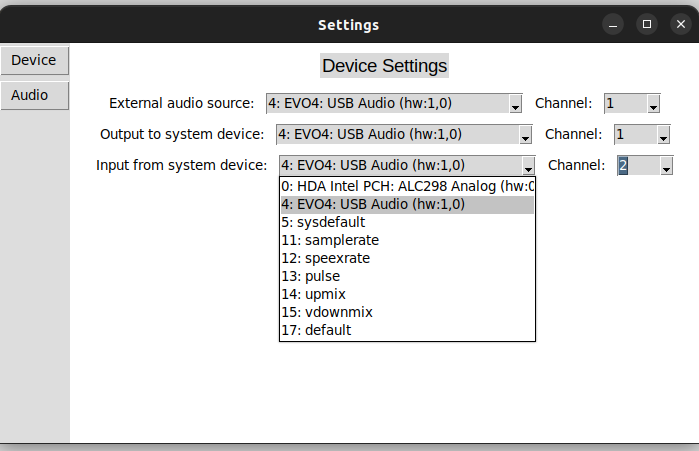
\includegraphics[width=0.8
	\linewidth]{Figures/Coro_Device_settings.png}
	\caption{Device Settings Window recognizing EVO 4 soundcard}
	\label{fig:Coro_device_settings}
\end{figure}

As we can see in Figure~\ref{fig:Coro_device_settings}, the program automatically recognized the \textit{EVO 4} soundcard without any prior configuration—just by plugging it in and setting the Device Settings window. At this point, I only changed the sample rate to 96 kHz from the Audio Settings page, confirming that the soundcard is compatible with this configuration. The other parameters were left at their default values.

Just to check if the parameters were working properly, I opened the RTA page, but something was not functioning correctly.

\begin{figure}[H]
	\centering
	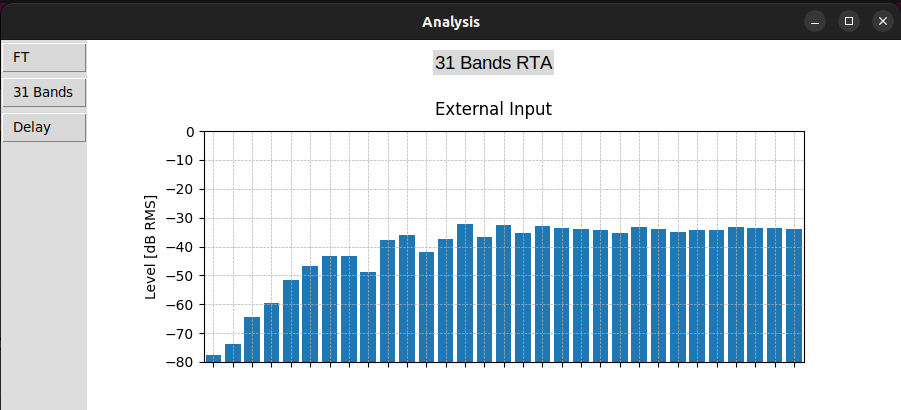
\includegraphics[width=0.8
	\linewidth]{Figures/Coro_Pink_Bad.png}
	\caption{First RTA measurement over the External Input}
	\label{fig:Coro_Bad_Pink}
\end{figure}

As shown in Figure~\ref{fig:Coro_Bad_Pink}, with pink noise coming from the \textbf{External Input}, the External Input analysis shows a lack of low-frequency energy. I suspected that this might be due to the block size parameter being too small at this sample rate (which means a short analysis time window). To achieve a better representation of low frequencies, I increased the block size parameter, as shown in Figure~\ref{fig:Coro_audio_settings}, to 16,384 samples per block.

\begin{figure}[H]
	\centering
	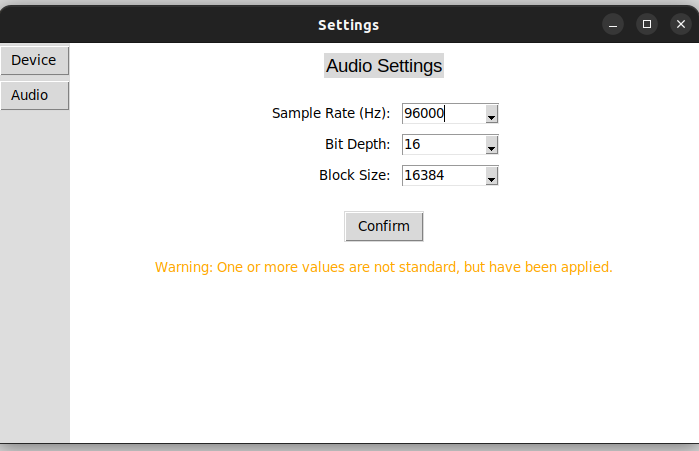
\includegraphics[width=0.8
	\linewidth]{Figures/Coro_audio_settings.png}
	\caption{Audio Settings Window after changes}
	\label{fig:Coro_audio_settings}
\end{figure}

This block size, at a 96 kHz sampling rate, represents 170.7 ms, which in the worst case corresponds to approximately 3.4 wavelengths at 20 Hz (the lowest frequency considered). With this  setting, we can observe in Figure~\ref{fig:Coro_Good_Pink} that the results are not perfect, but much better. I considered them good enough for this test.

\begin{figure}[H]
	\centering
	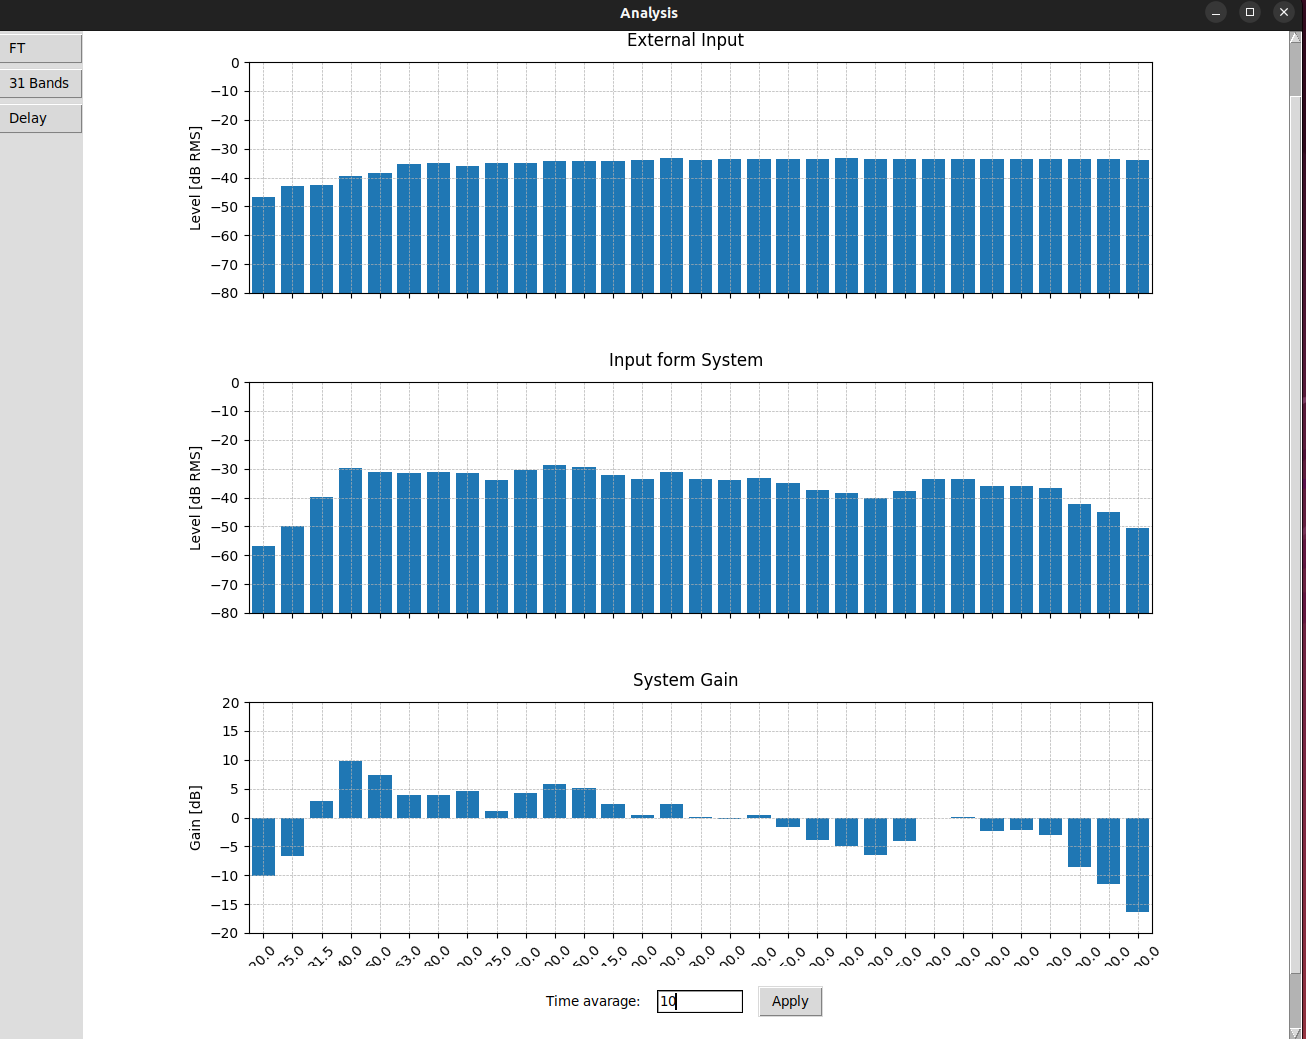
\includegraphics[width=0.8
	\linewidth]{Figures/Coro_Pink_Good.png}
	\caption{Second RTA measurement over the External Input}
	\label{fig:Coro_Good_Pink}
\end{figure}

Once this was working properly, I started measuring the delay, which should correspond to the time it takes for sound to travel from the speaker to the microphone. Considering the speed of sound as 340 m/s, this value should represent the distance between the two devices.

\begin{figure}[H]
	\centering
	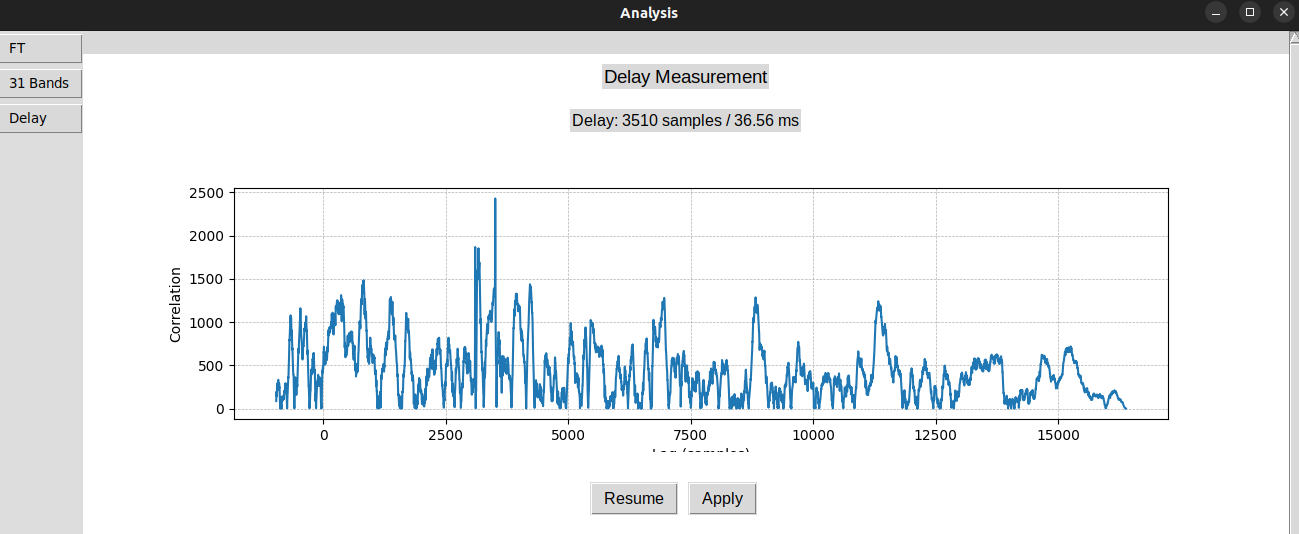
\includegraphics[width=0.8
	\linewidth]{Figures/Coro_Delay.png}
	\caption{First Delay Measurement}
	\label{fig:Coro_delay1}
\end{figure}

The measurement was not very stable—most iterations gave different values. However, I paused the process and took the most consistent and frequently repeated value. Additionally, I considered the correlation plot to ensure the result was reliable, focusing on cases where the maximum value clearly stood out from the rest. This can be seen in Figure~\ref{fig:Coro_delay1}. 

The measured delay was 36.56 ms, which—considering the speed of sound (340 m/s)—corresponds to a distance of 12.43 m. However, as shown in Figure~\ref{fig:spk-mic}, the actual physical distance between the speaker and the microphone is 8.86 m, which is 3.57 m more than expected.

It is logical to expect a slightly longer delay than the pure acoustic distance, since the signal passes through various systems before reaching the speaker—each of which may introduce some latency. For example, it is known that the mixing console adds approximately 0.3 ms of latency per output channel, which corresponds to only 0.1 m of additional delay. Even if this latency accumulates through multiple stages, it is still not enough to justify the extra 3.57 m (around 10.5 ms).

Because of this significant discrepancy, I continued measuring to investigate further.

\begin{figure}[H]
	\centering
	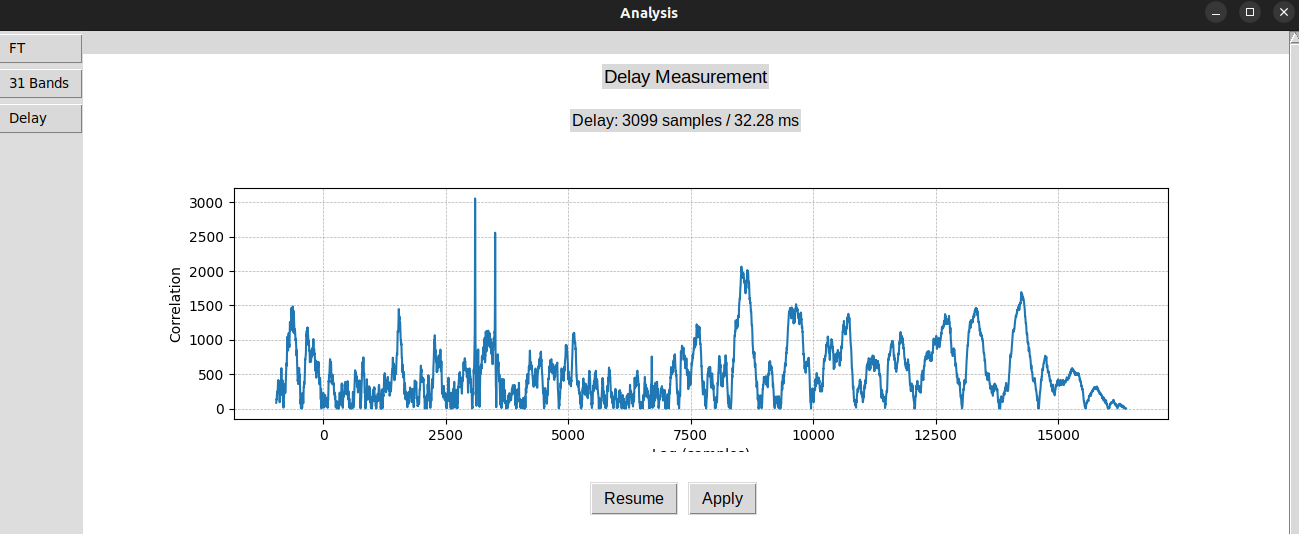
\includegraphics[width=0.8
	\linewidth]{Figures/Coro_delay_2.png}
	\caption{Second Delay Measurement}
	\label{fig:Coro_delay2}
\end{figure}

After observing the iterations of the plot and the measurement results for a while, I realized that there was a second value that appeared repeatedly across many iterations and also made sense visually on the plot. As shown in Figure~\ref{fig:Coro_delay2}, the plot clearly highlights two peaks with significant correlation values. At the right moment I stopped the measurement, the lower time value among the two had the highest correlation, which corresponded to 32.28 ms. This value translates to a distance of 10.98 m, which is 2.12 m more than the actual physical distance between the speaker and the microphone.

Although not fully conclusive, this second measurement seems more reasonable than the previous one, so I decided to use this value and apply it over the rest of the measurements.

Next step is open the FT page.

\begin{figure}[H]
	\centering
	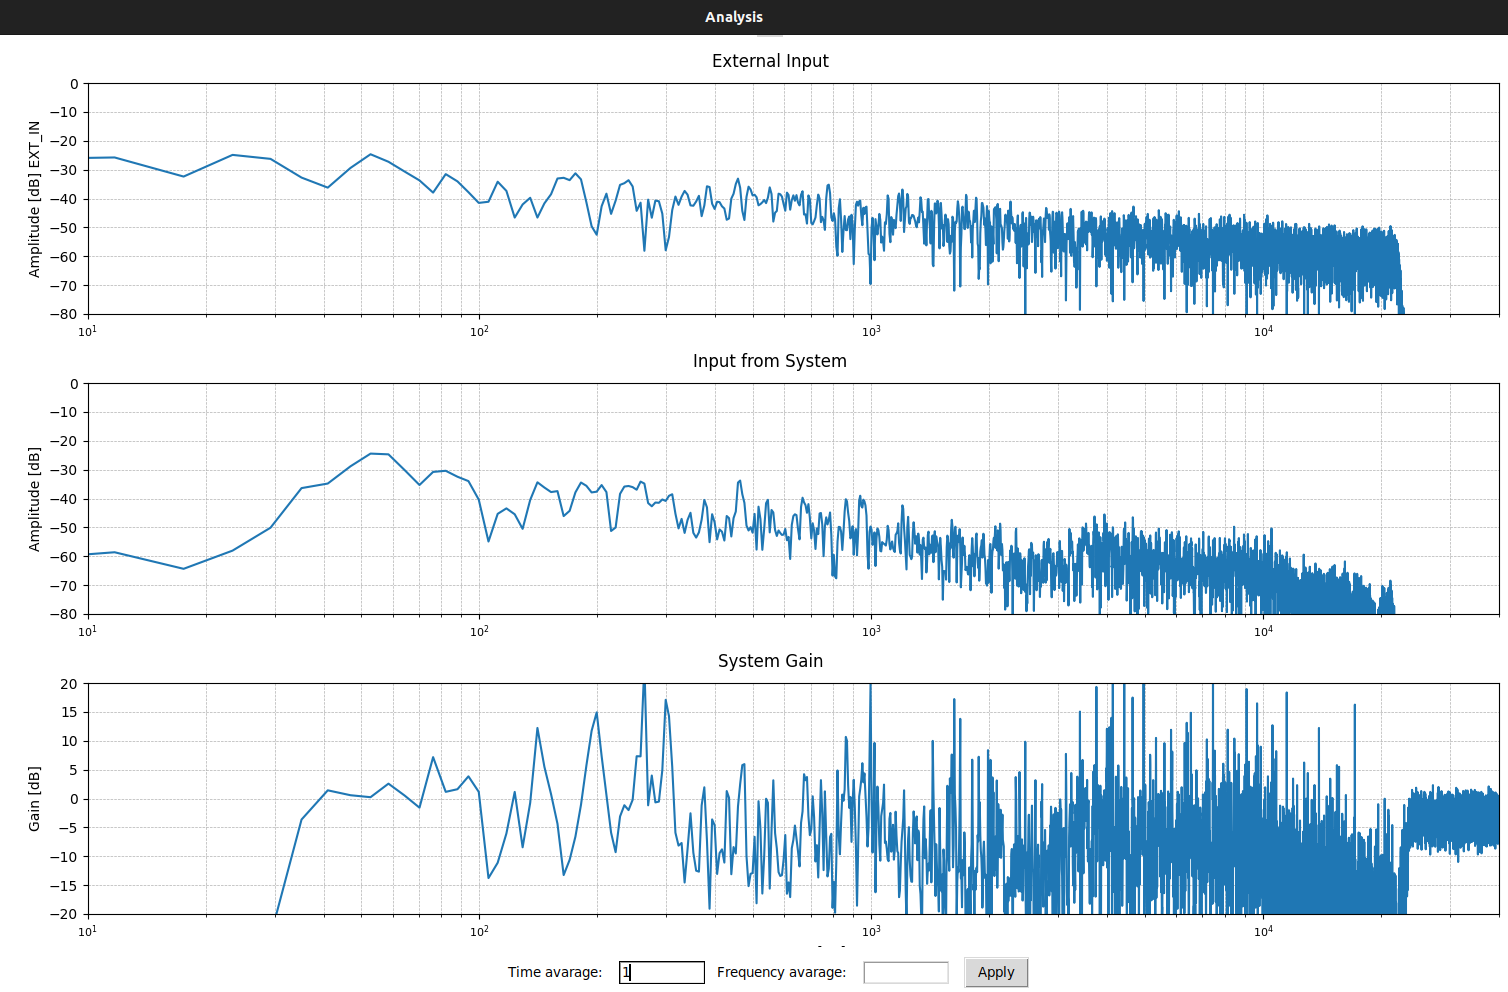
\includegraphics[width=0.8
	\linewidth]{Figures/Coro_FT_NO_av.png}
	\caption{FT Measurement Without Averaging Applied}
	\label{fig:Coro_FT_no_av}
\end{figure}

Continuing with Pink noise excitation from \textbf{External Input}. I can see the FT page results without applying any avarage option, as shown on Figure~\ref{fig:Coro_FT_no_av}. But the plots are very anarchic, changes a lot between iterations, and is difficult to make a solid interpretaion.

\begin{figure}[H]
	\centering
	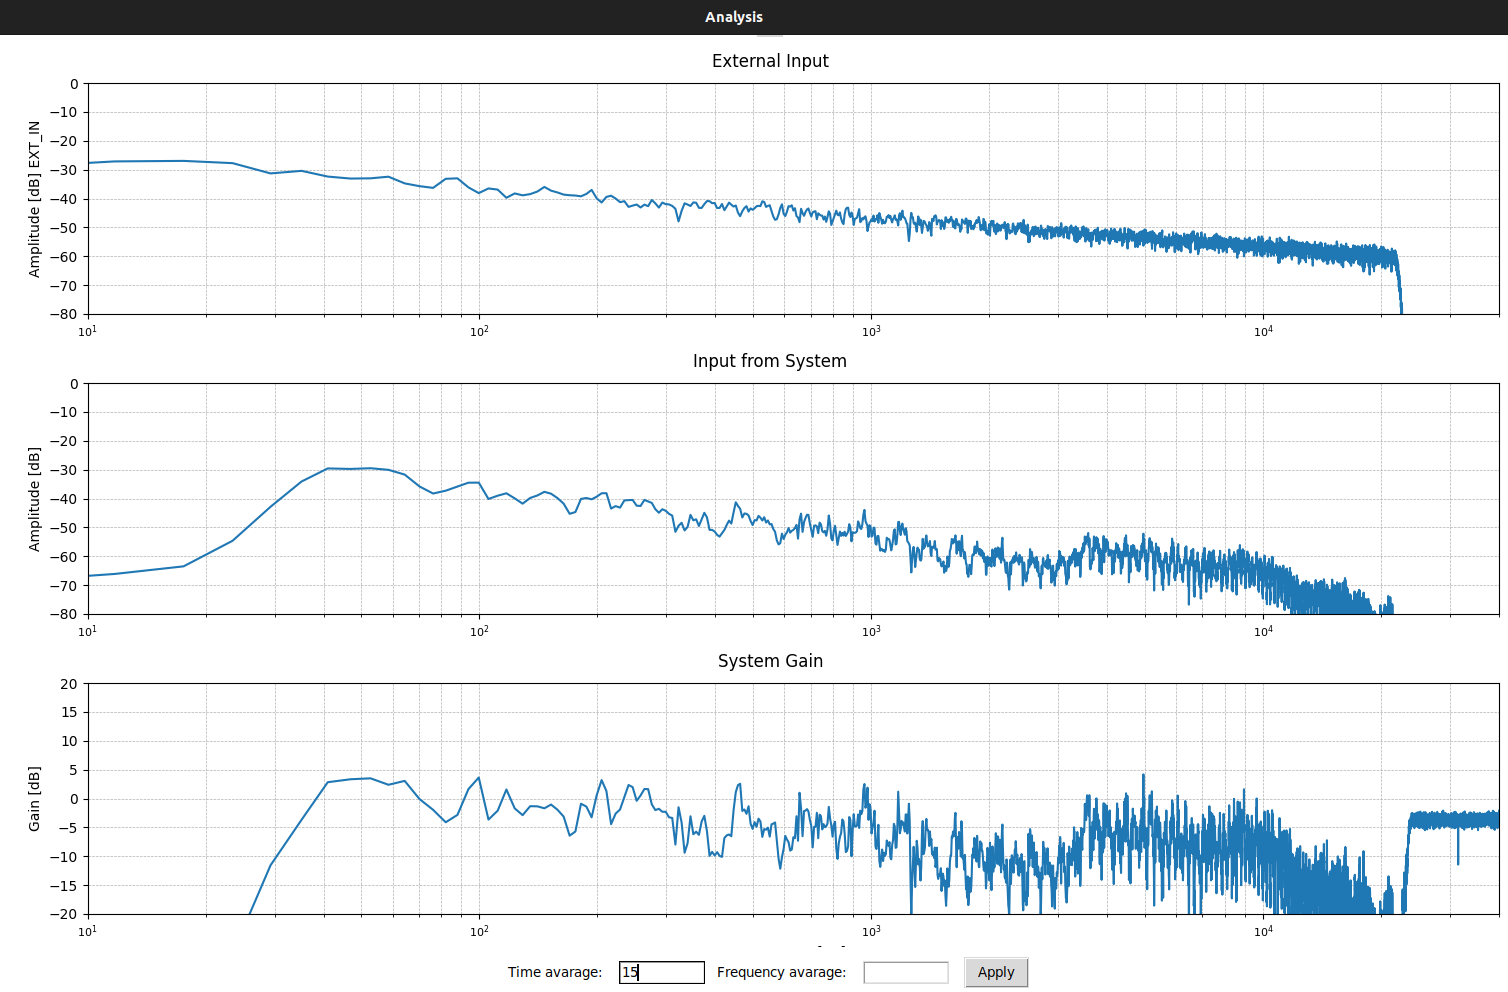
\includegraphics[width=0.8
	\linewidth]{Figures/Coro_FT_time_av.png}
	\caption{FT Measurement With Time Averaging Applied}
	\label{fig:Coro_FT_time_av}
\end{figure}

In Figure~\ref{fig:Coro_FT_time_av}, a time average is applied, which greatly improves the consistency between iterations and makes it much easier to interpret the displayed data. However, interpreting the data in the high-frequency range is still somewhat confusing. To address this, I applied frequency averaging.

\begin{figure}[H]
	\centering
	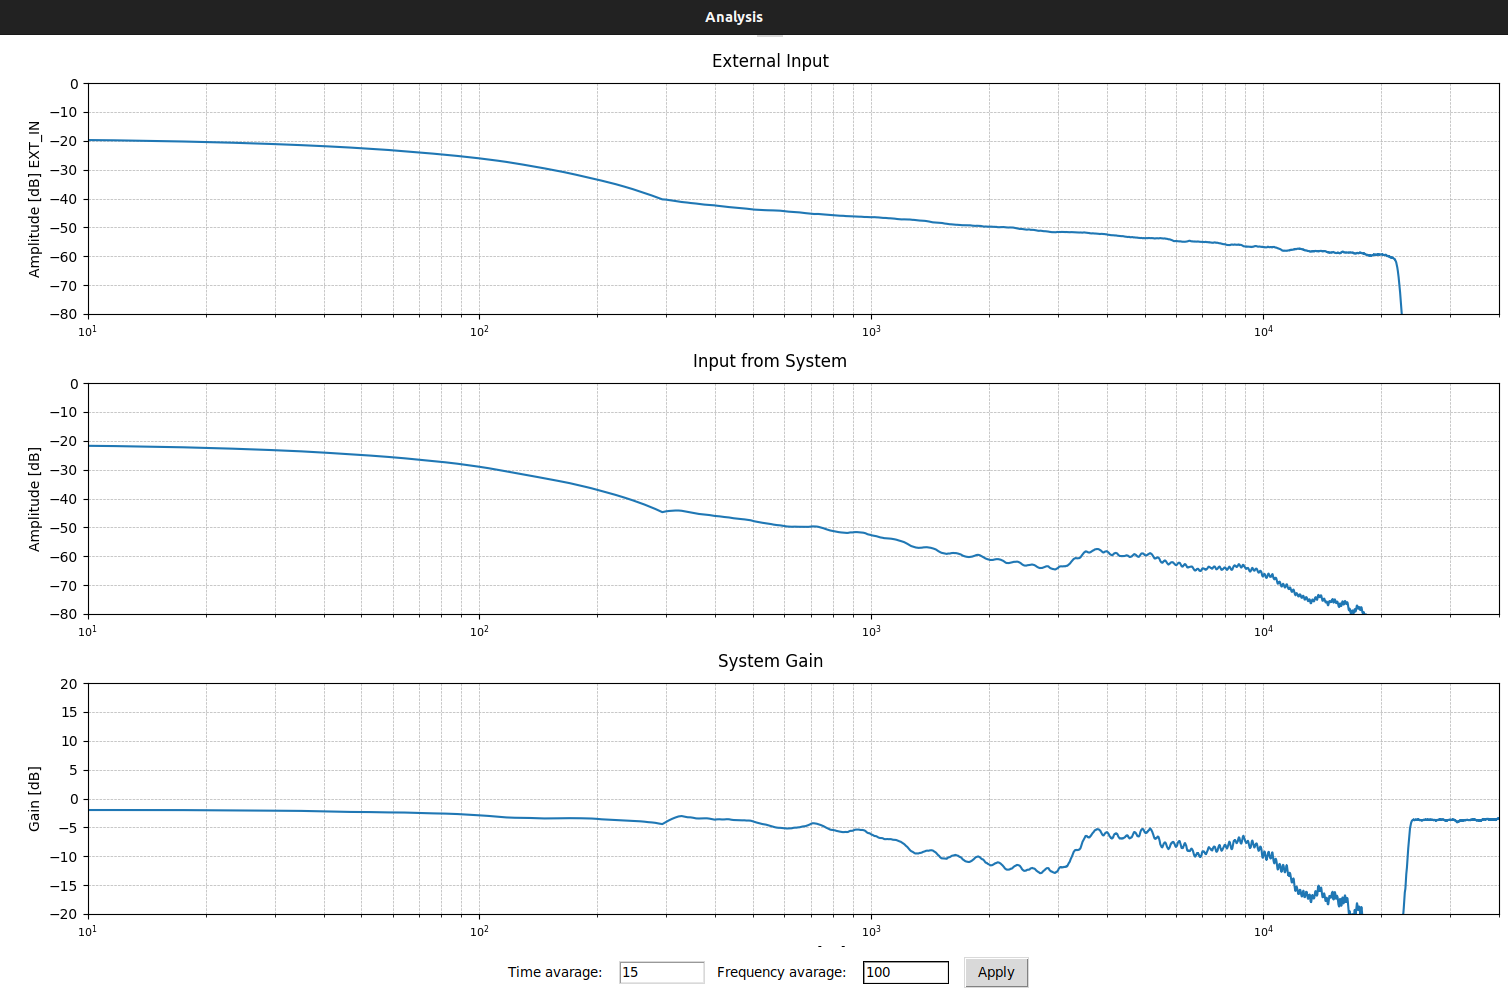
\includegraphics[width=0.8
	\linewidth]{Figures/Coro_FT_WITH_av.png}
	\caption{FT Measurement with Time and Frequency Averaging Applied}
	\label{fig:Coro_FT_av}
\end{figure}

With all averaging options applied, we obtain the result shown in Figure~\ref{fig:Coro_FT_av}. While we lose considerable resolution in the low-frequency range, the high-frequency representation becomes much more visually understandable.

\begin{figure}[H]
	\centering
	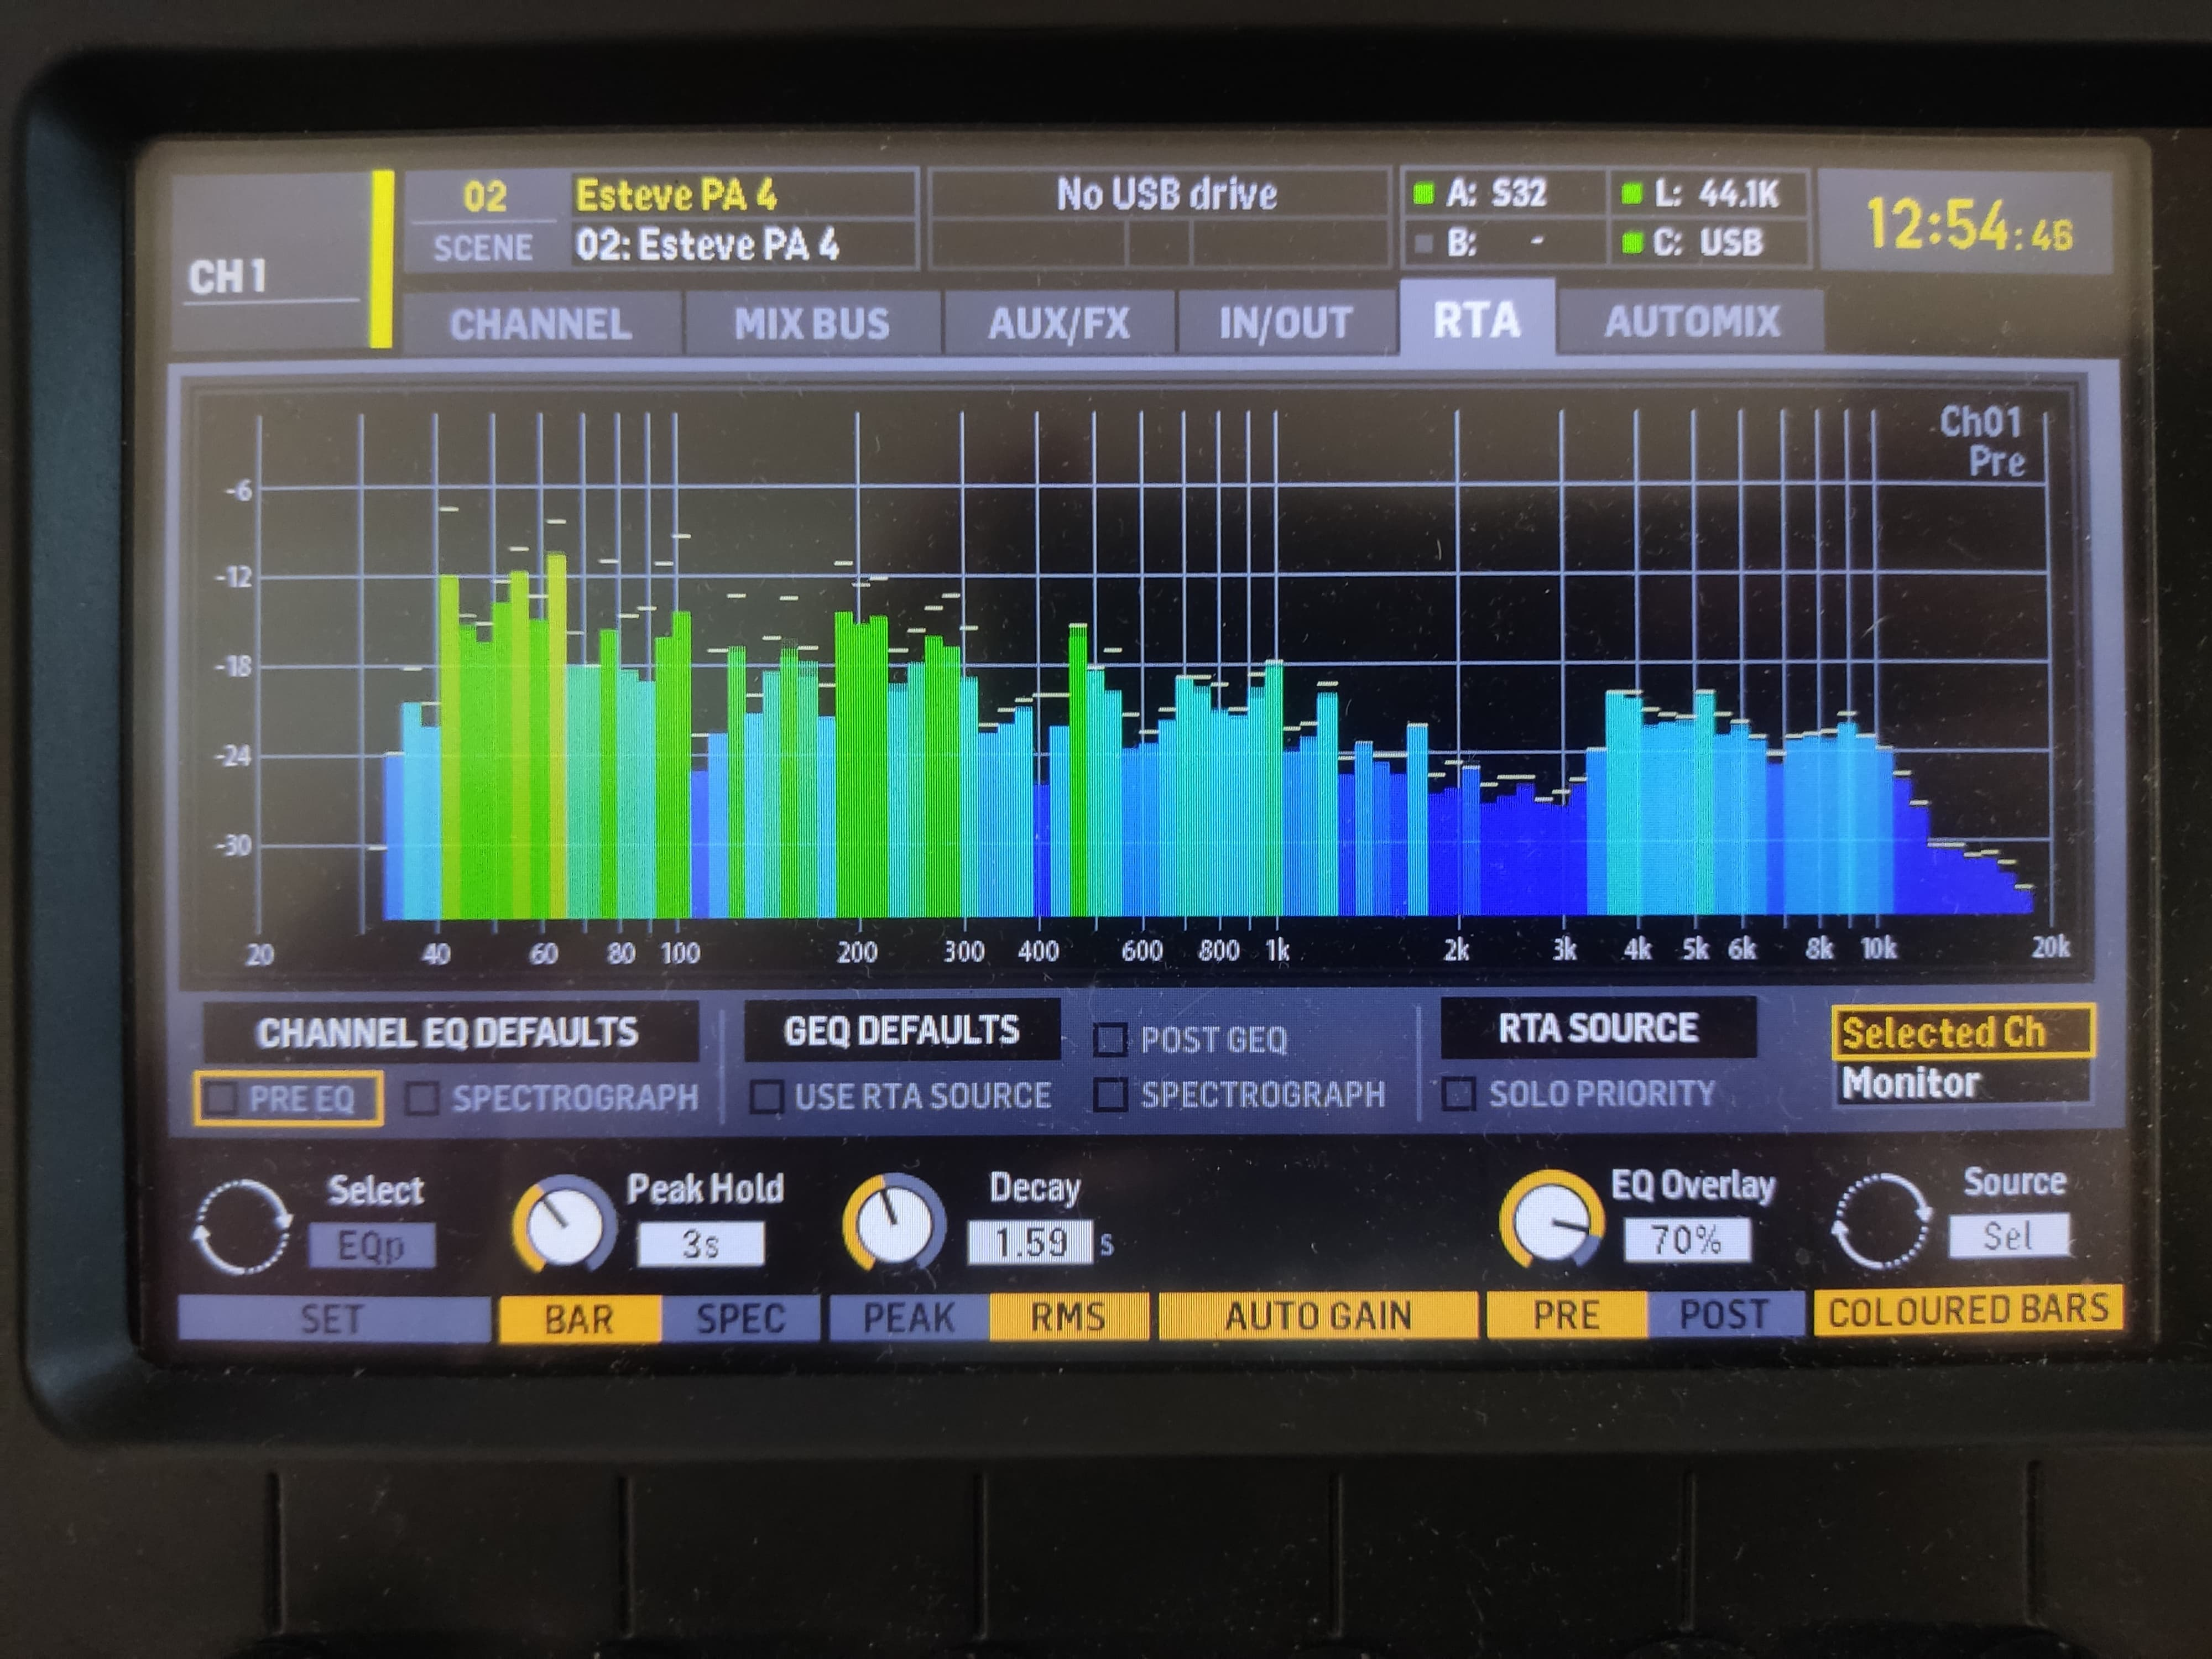
\includegraphics[width=0.8
	\linewidth]{Figures/Coro_X32_nontreated.jpeg}
	\caption{X32 RTA Tool with Untreated Input from System Signal}
	\label{fig:Coro_X32_nontreated}
\end{figure}

To check whether the results are reasonably close to reality, we use the \textbf{X32} RTA tool as a reference and compare it with the \textbf{Input from System} analysis. As shown in Figure~\ref{fig:Coro_X32_nontreated}, and comparing it with the FT page of the RTA+C program (see previous figures), the results look very similar—especially the dip between 1000 Hz and 4000 Hz. Therefore, I consider that the FT page works pretty well.

Next step: open the RTA page.

\begin{figure}[H]
	\centering
	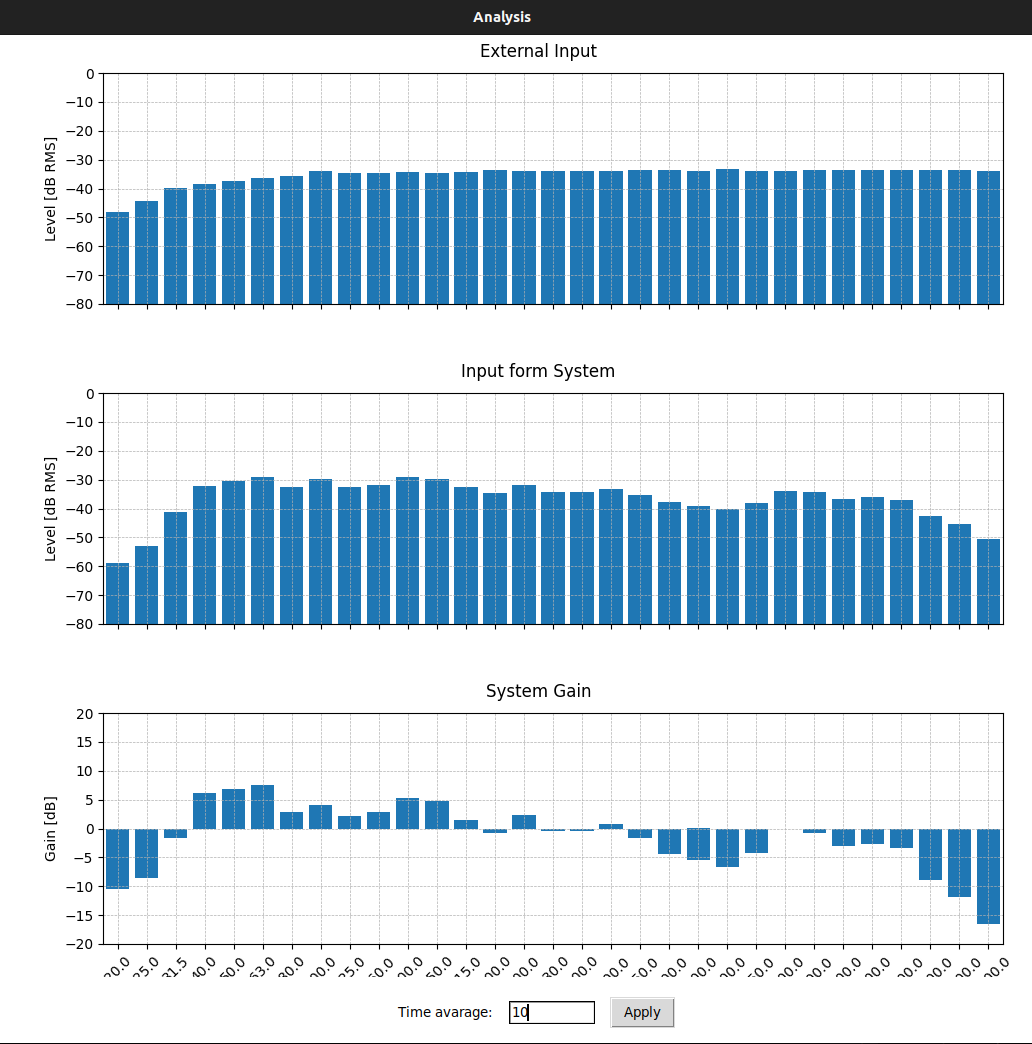
\includegraphics[width=0.8
	\linewidth]{Figures/Coro_RTA_Saved.png}
	\caption{Reference RTA values, saved to apply in the Correction Window}
	\label{fig:Coro_RTA_saved}
\end{figure}

Referencing Figure~\ref{fig:Coro_RTA_saved}, with 10 iterations averaged, I obtained a reasonably stable plot that is easy to interpret. Additionally, when compared with Figure~\ref{fig:Coro_X32_nontreated}, we can clearly observe similarities with the \textbf{Input from System} analysis. The plot also accurately displays a flat response for the \textbf{External Input}, which is expected given that this signal is a clean Pink Noise.

Considering these results satisfactory, I saved the \textbf{System Gain} values using the "\textit{Save Gain}" button. Now, it's time to open the \textbf{DSP} window.

\begin{figure}[H]
	\centering
	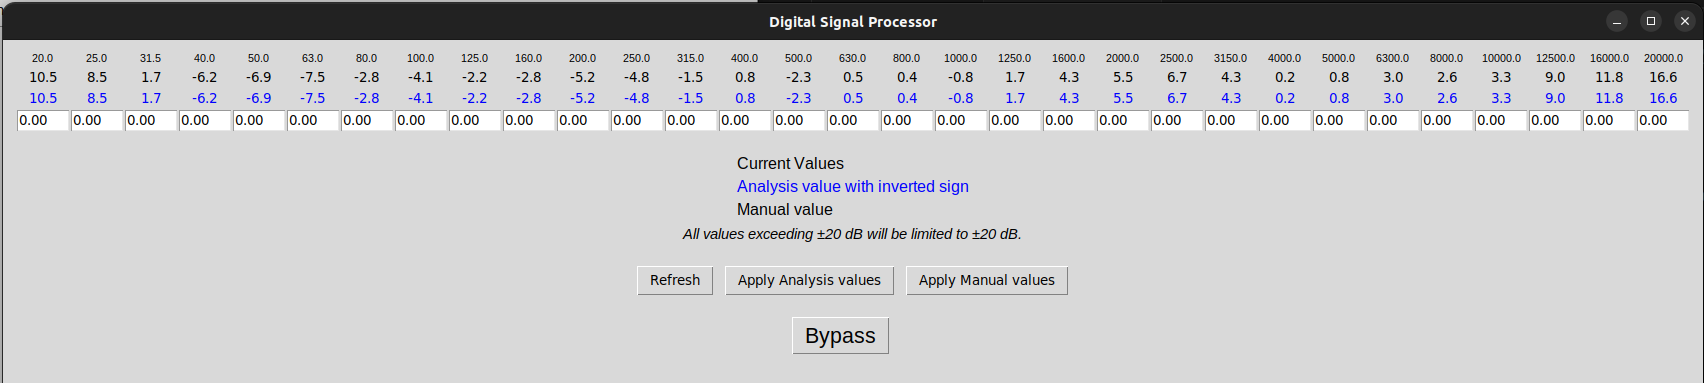
\includegraphics[width=1
	\linewidth]{Figures/Coro_EQ_from_RTA.png}
	\caption{DSP window with EQ values applied from RTA analysis}
	\label{fig:Coro_EQ_RTA+C}
\end{figure}

Once the \textbf{DSP} window is opened, since the values from the RTA were previously saved, it automatically loads with the \textit{Analysis Values} imported with inverted sign (to apply correction, we need to compensate the analysis values, which is done by inverting their sign). If we overwrite the saved ones, or if there were no values when this page was first opened, it is possible to import the latest saved values using the \textit{Refresh} button. Then, simply press \textit{Apply Analysis values} to send them to the \textbf{EQ} modules. At this point, the page is configured as shown in Figure~\ref{fig:Coro_EQ_RTA+C}. Additionally, it is also possible to manually enter values; in that case, pressing the \textit{Apply Manual values} button will activate them.

At this point, I deactivated the \textbf{X32} Bypass to activate the EQ module from the RTA+C program with the applied values. Luckily, with pink noise, the glitch effect is almost unnoticeable.

\begin{figure}[H]
	\centering
	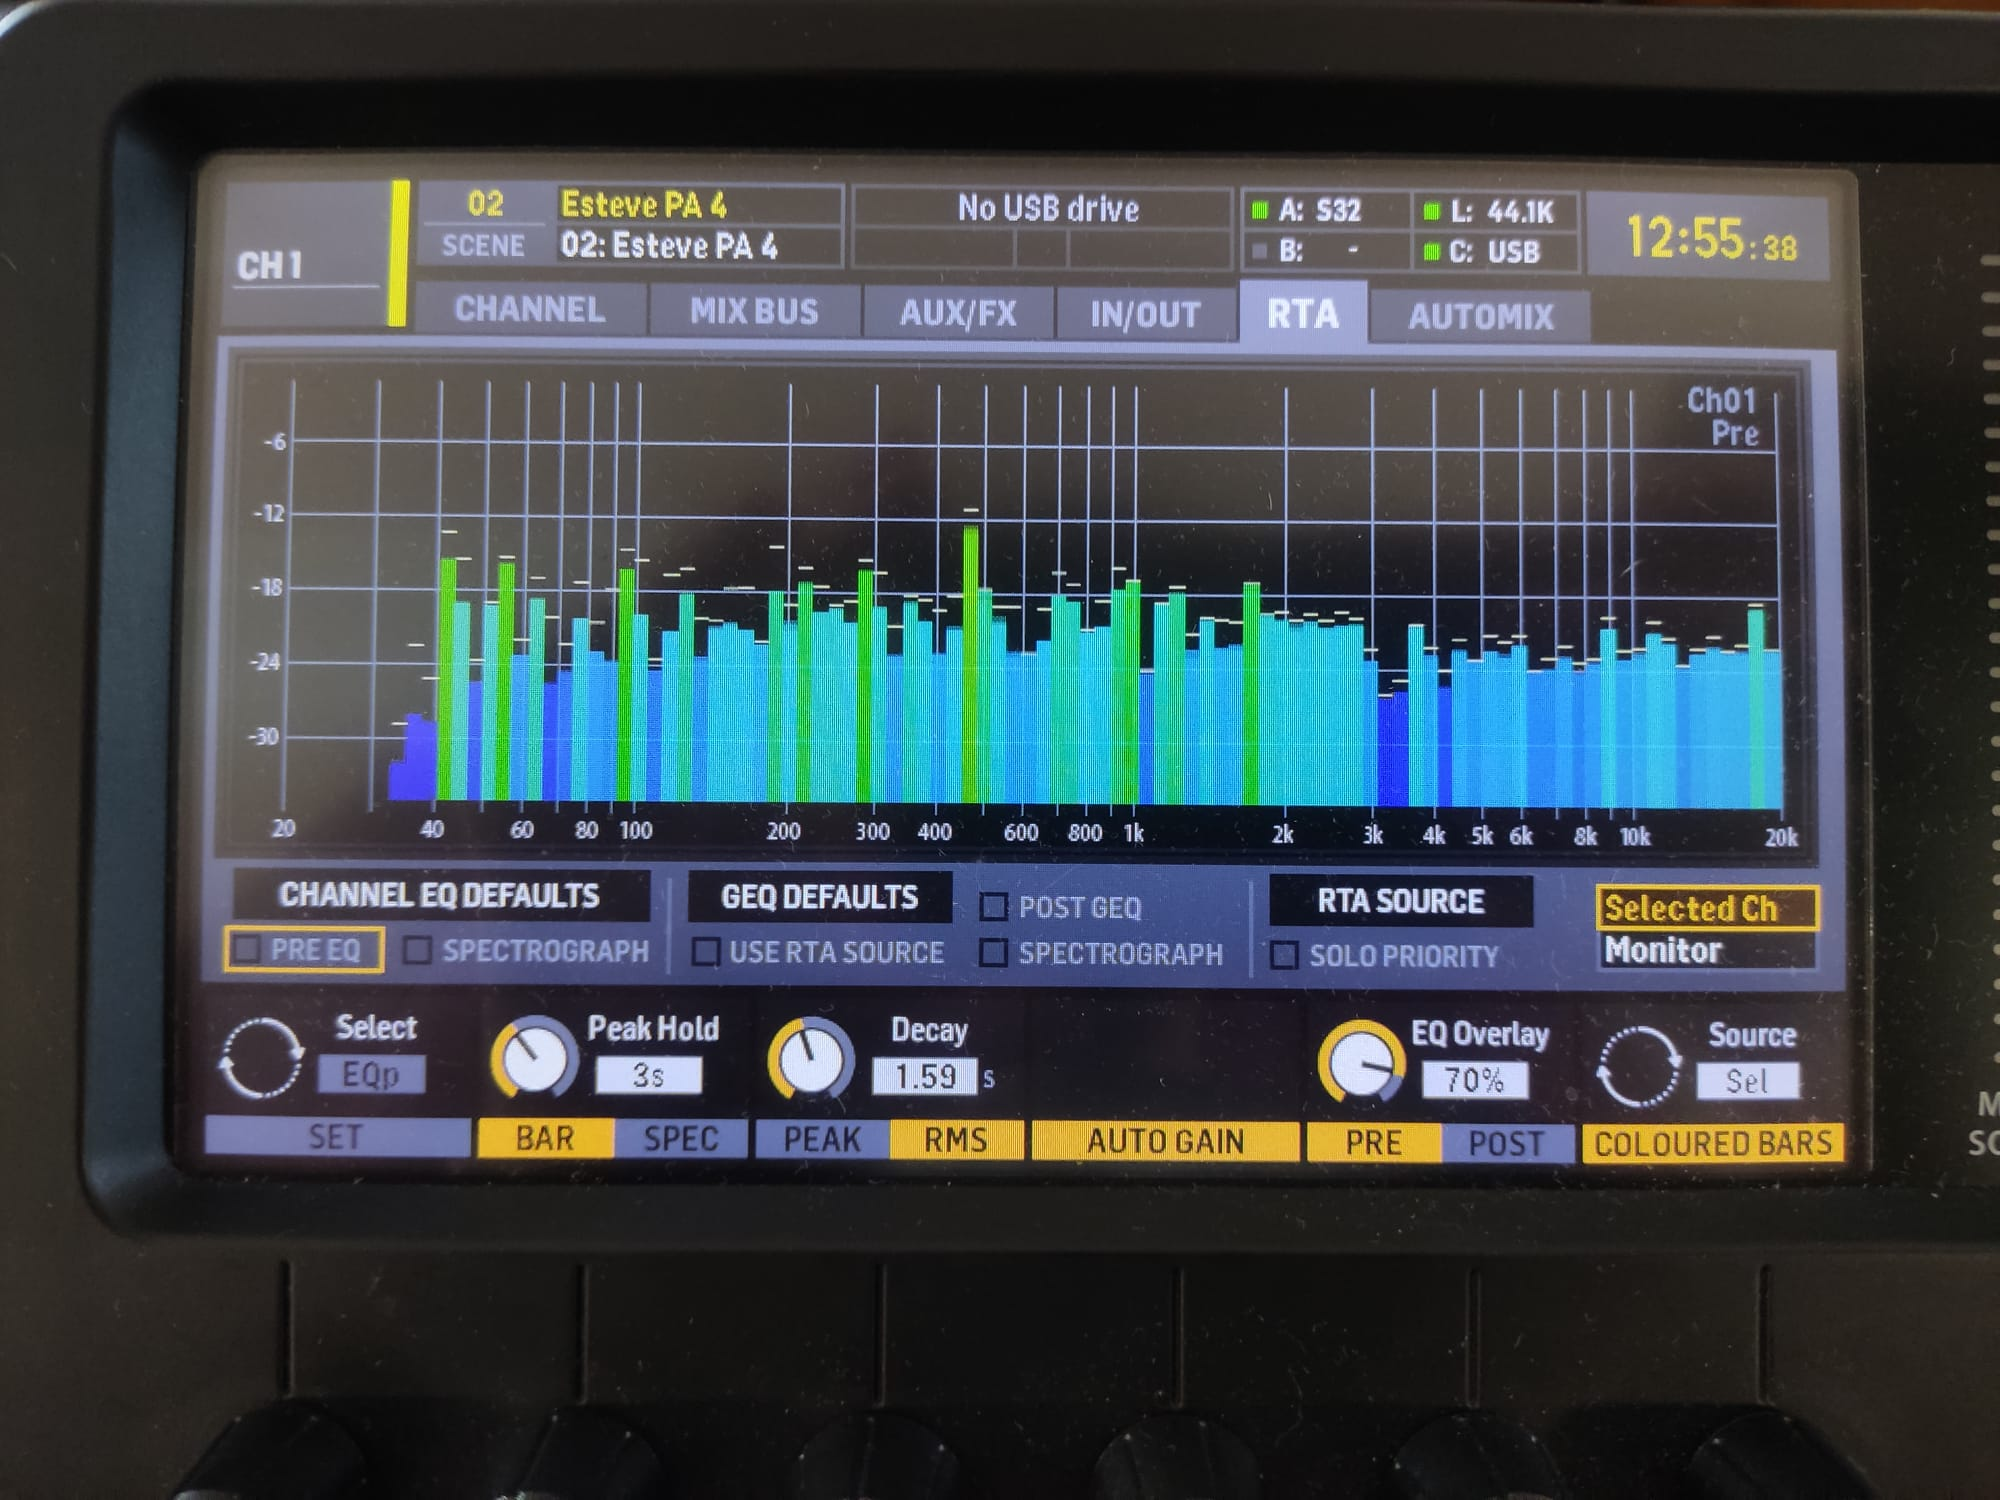
\includegraphics[width=0.8
	\linewidth]{Figures/Coro_X32_treatedRTAc.jpeg}
	\caption{X32 RTA tool with Treated Input form System Signal}
	\label{fig:Coro_X32_RTA+C}
\end{figure}

First, I took a look at the \textbf{X32} RTA tool, shown in Figure~\ref{fig:Coro_X32_RTA+C}, to compare it with the non-correction applied results from Figure~\ref{fig:Coro_X32_nontreated}. Clearly, the graph looks flatter, which indicates that the correction is working properly and yielding good results. It’s not perfect, but the dip between 1000 and 4000 Hz has improved significantly.

\begin{figure}[H]
	\centering
	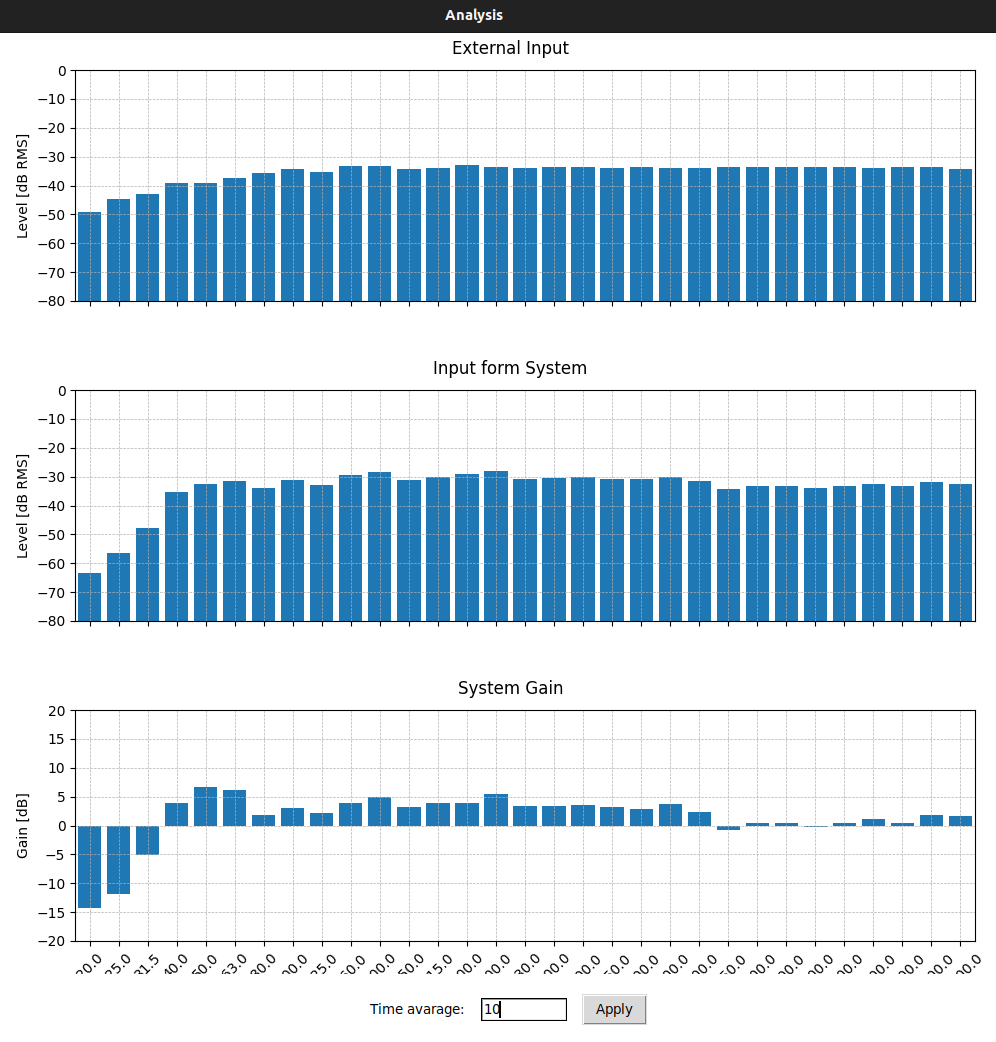
\includegraphics[width=0.8
	\linewidth]{Figures/Coro_RTA+EQ_ON.png}
	\caption{RTA Results After Activating RTA+C EQ}
	\label{fig:Coro_RTA_RTA+C}
\end{figure}

Then, I looked at the RTA module page from \textbf{RTA+C}, shown in Figure~\ref{fig:Coro_RTA_RTA+C}, and the results looked very promising. The plot appeared much flatter compared to previous measurements, which indicates that the EQ module is functioning correctly. This also confirms that using the same filters for both analysis and processing was a good design choice. What remains pending is further research and the implementation of improved filters to achieve a more natural and realistic representation of the real acoustic response.

\begin{figure}[H]
	\centering
	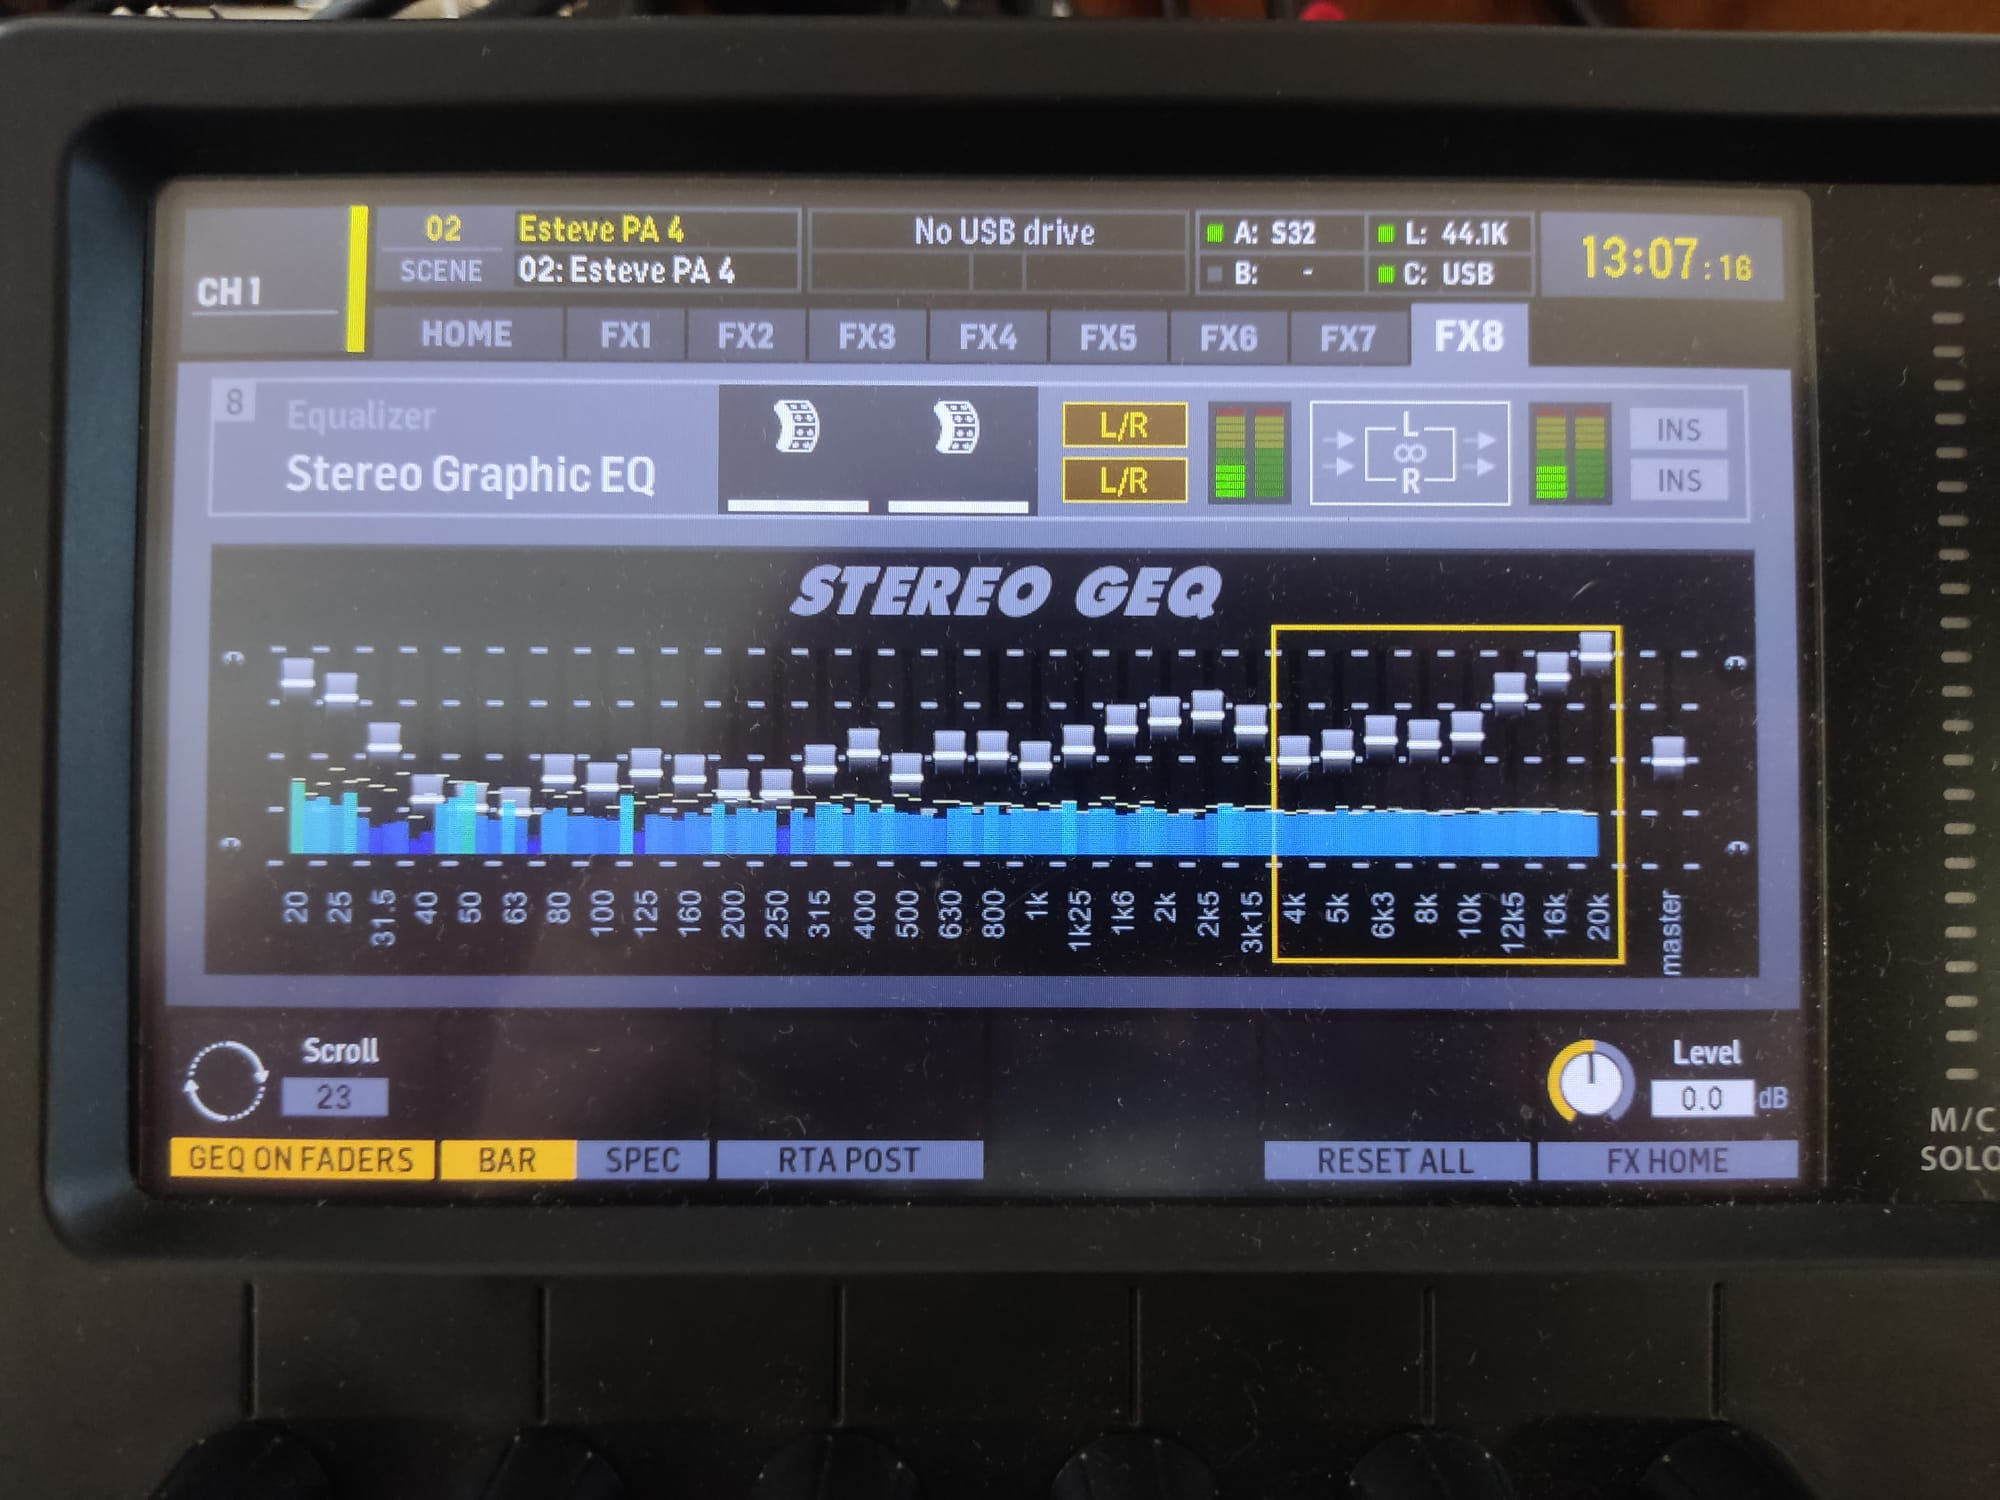
\includegraphics[width=0.8
	\linewidth]{Figures/Coro_X32_EQ.jpeg}
	\caption{Configuring the X32 EQ tool with parameters obtained from RTA+C}
	\label{fig:Coro_X32_EQ}
\end{figure}

Also, I wanted to compare the correction applied by \textbf{RTA+C} with the \textit{Stereo GEQ} tool of the \textbf{X32} console. To do so, I configured the console's EQ tool with the same parameters used in the EQ module of the software (taken directly from the RTA page of \textbf{RTA+C}). The configuration is shown in Figure~\ref{fig:Coro_X32_EQ}.

\begin{figure}[H]
	\centering
	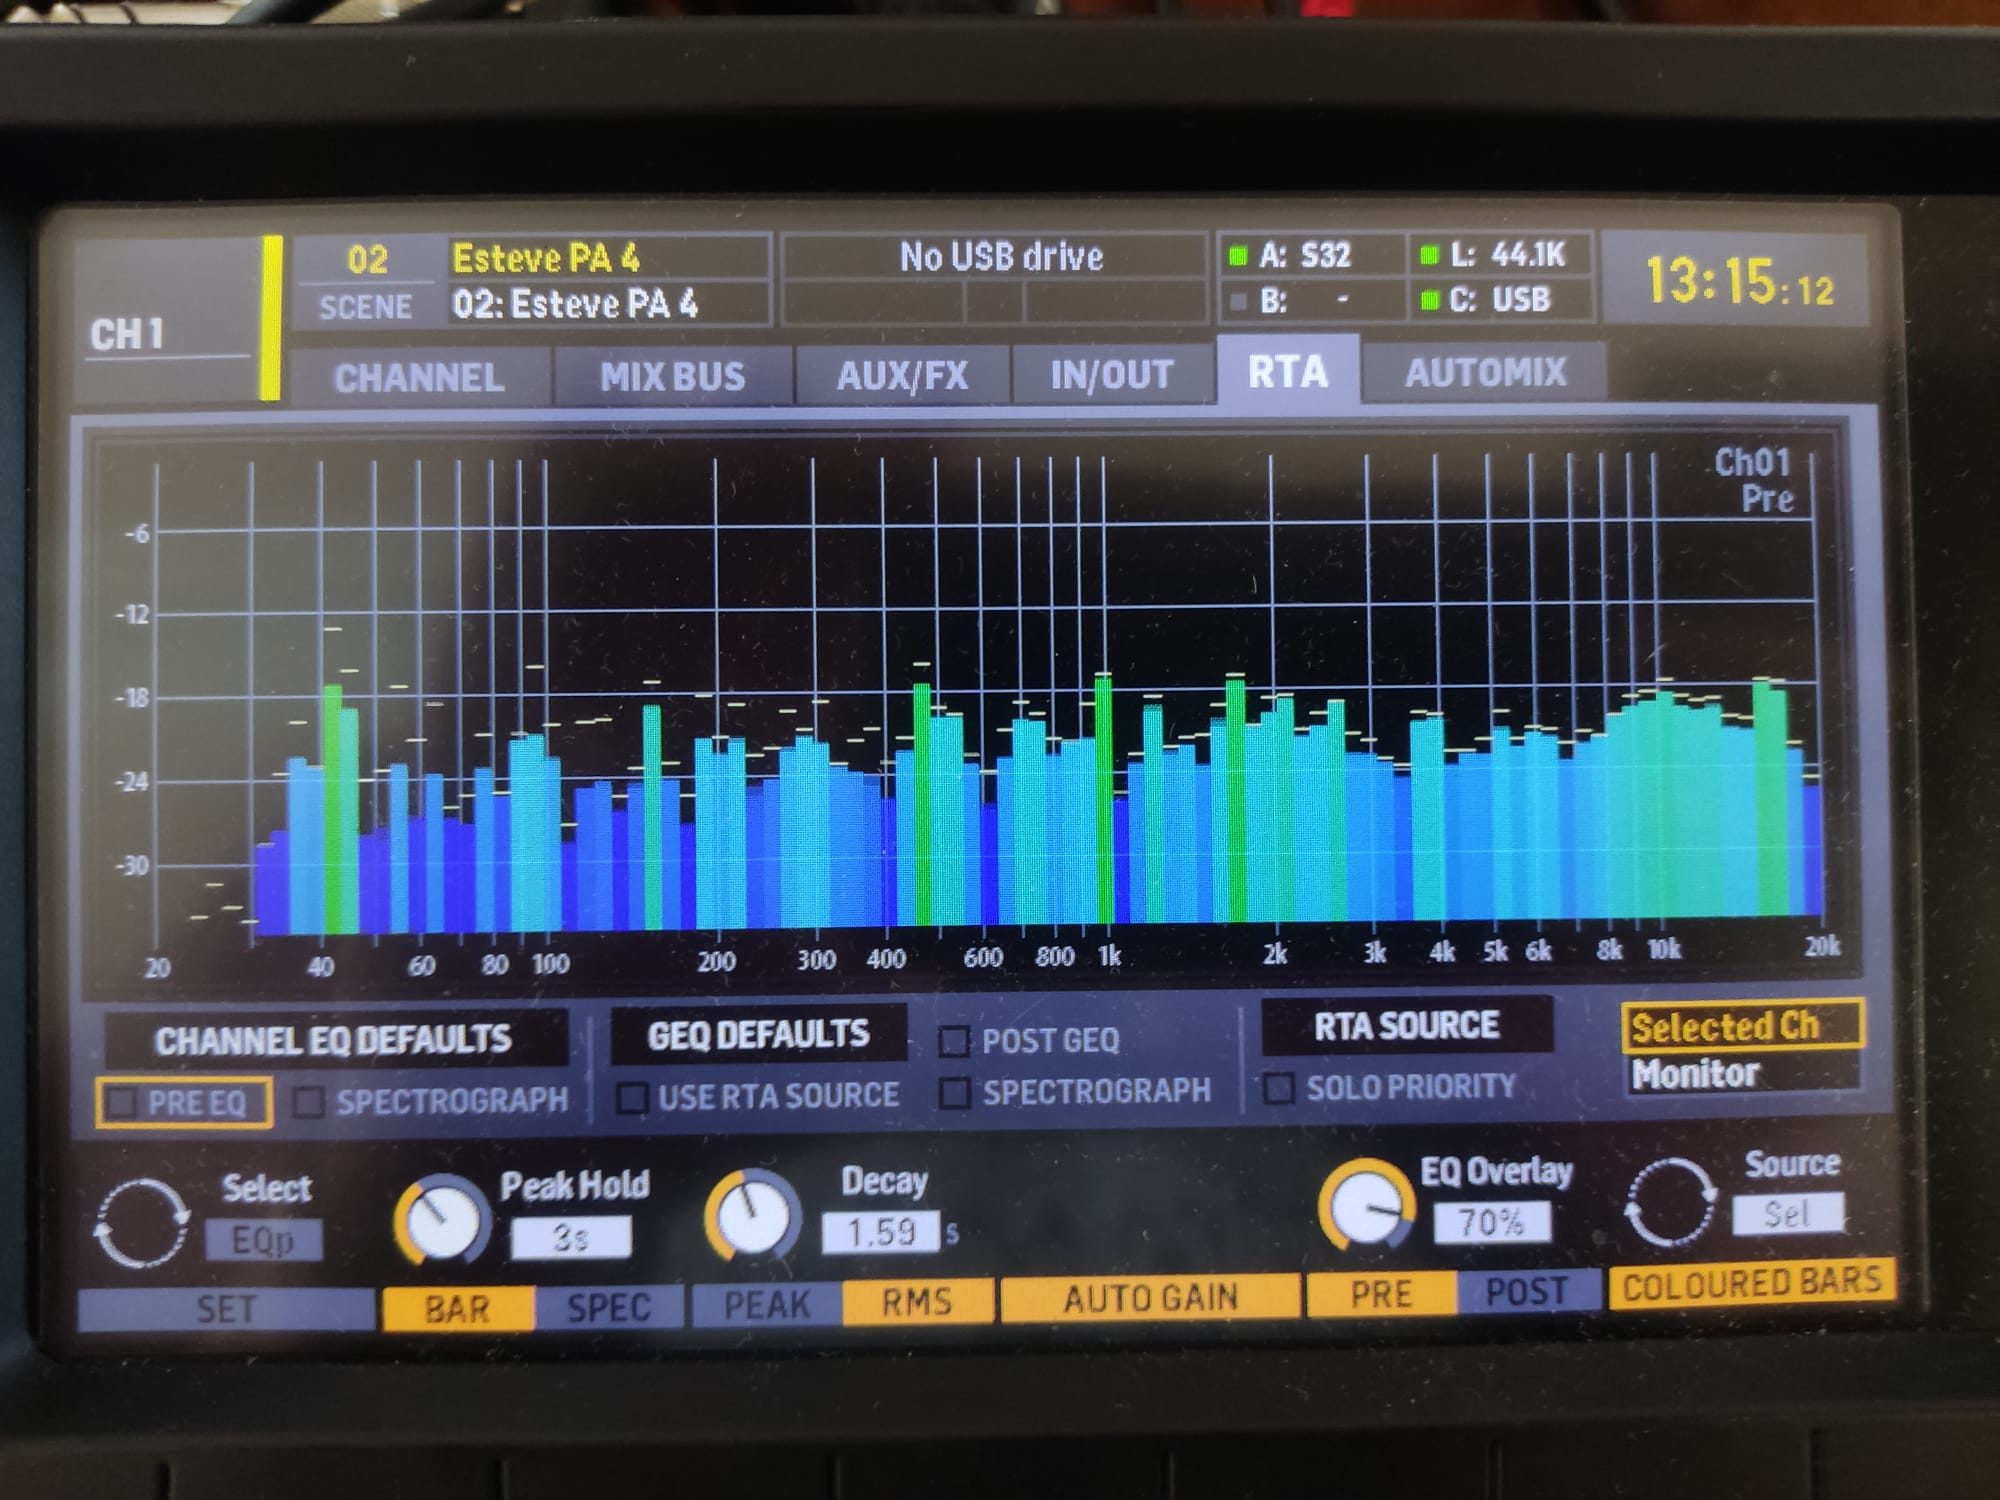
\includegraphics[width=0.8
	\linewidth]{Figures/Coro_X32_treatedX32.jpeg}
	\caption{Input from System with X32 EQ treatment, visualized using X32 RTA tool}
	\label{fig:Coro_X32_treatedX32}
\end{figure}

And in Figure~\ref{fig:Coro_X32_treatedX32}, we can see the \textbf{Input from System} signal displayed by the RTA tool of the \textbf{X32} console. This result was obtained after processing the \textbf{Output to System} signal with the console's \texttt{Stereo GEQ} tool using the same parameters taken from the \textbf{RTA+C} program. The result looks pretty good, and when comparing it with Figure~\ref{fig:Coro_X32_RTA+C}, the response is very similar. This suggests that the filters currently used in the \textbf{RTA+C} program are quite effective.

As I was testing a software solution intended to work properly in live situations, for the final test I replaced the pink noise with music.

\begin{figure}[H]
	\centering
	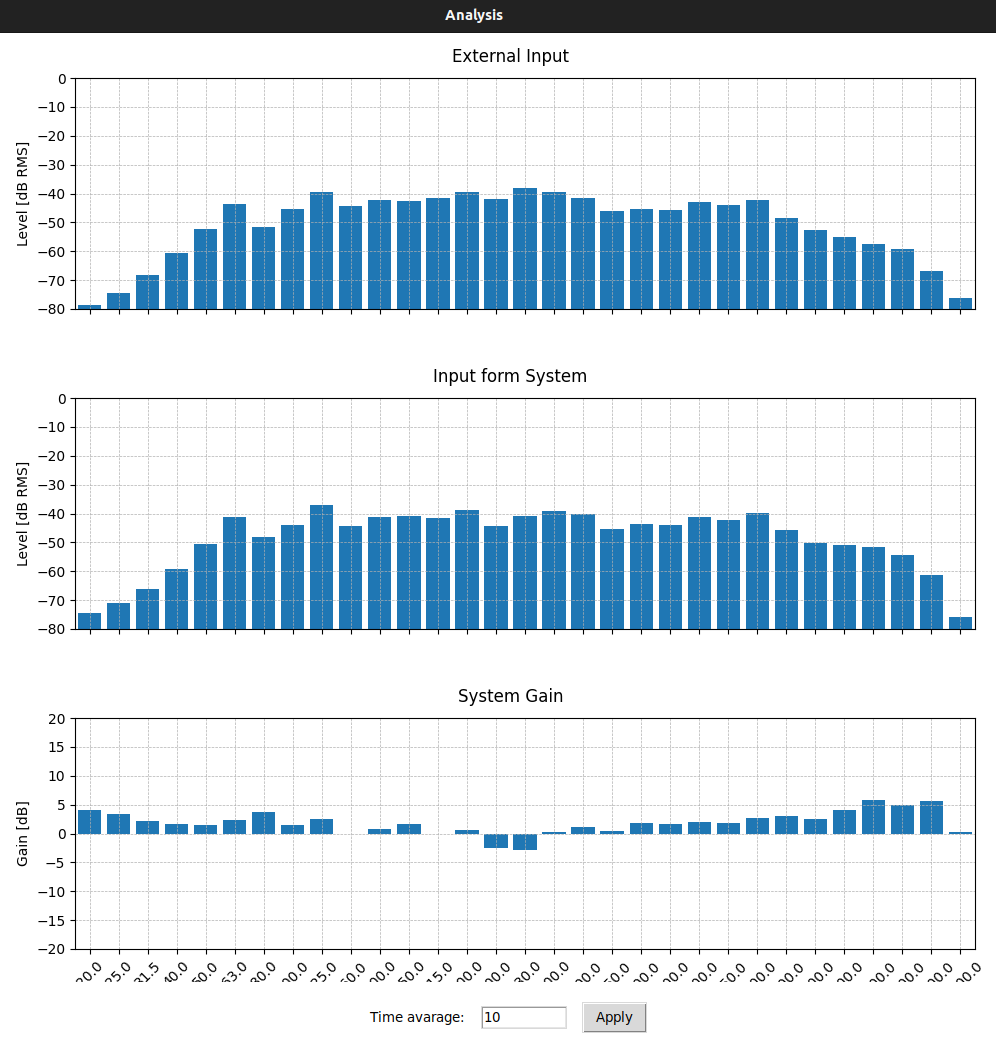
\includegraphics[width=0.8
	\linewidth]{Figures/Coro_Music_EQ_X32.png}
	\caption{RTA page, using music instead of pink noise}
	\label{fig:Coro_RTA_music}
\end{figure}

\begin{figure}[H]
	\centering
	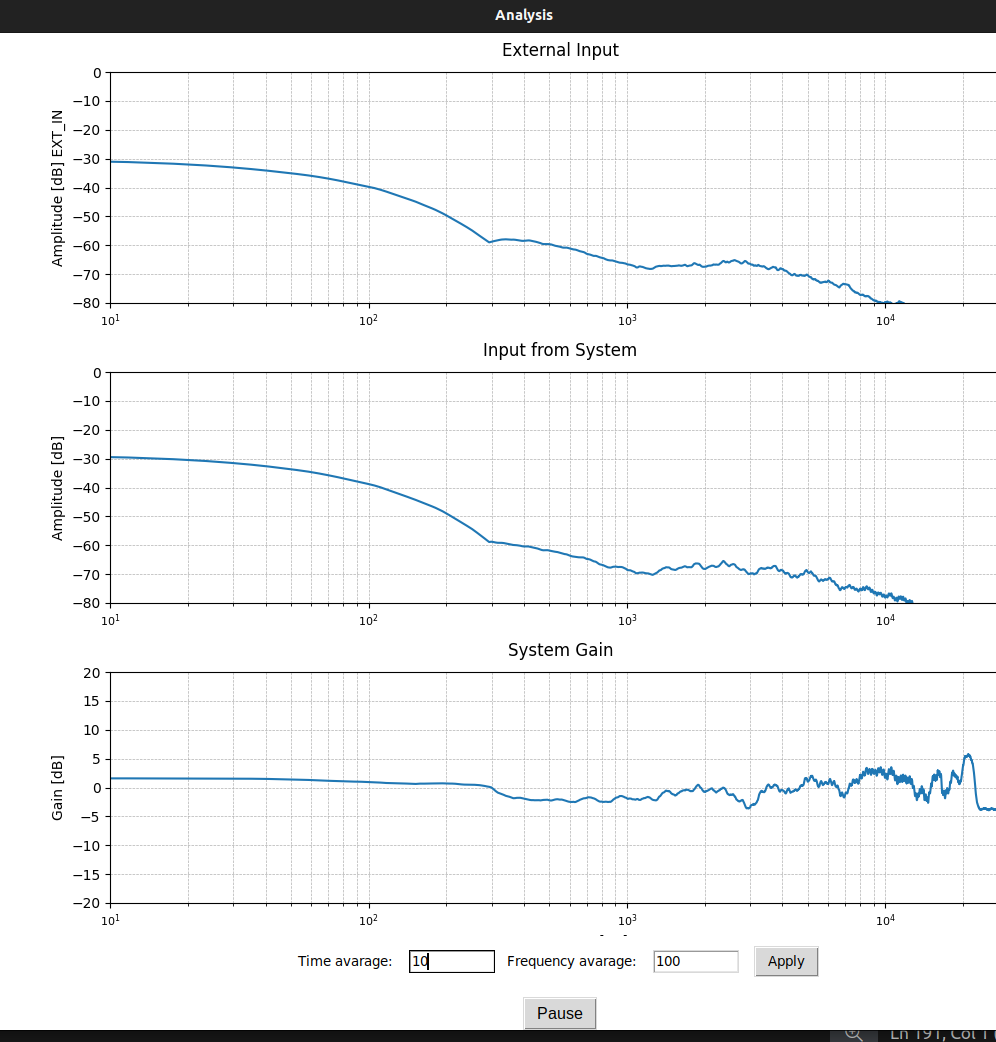
\includegraphics[width=0.8
	\linewidth]{Figures/Coro_FT_music_EQX32.png}
	\caption{FT page, using music instead of pink noise}
	\label{fig:Coro_FT_music}
\end{figure}

Using music and ignoring the glitch issue, I obtained the results shown in Figures~\ref{fig:Coro_RTA_music} and~\ref{fig:Coro_FT_music}. It was necessary to apply some averaging to make the results more understandable. Even so, the system performed quite well: although both the \textbf{External Input} and \textbf{Input from System} signals are constantly changing, the System Gain plots show only minor variations— which makes sense, since the analyzed system remains unchanged despite the music content varying. Moreover, because these signals are synchronized using the delay adjustment, the averaged results from different signal frames consistently represent the same slice of music.

Despite significant issues such as signal desynchronization (which causes glitch effects) and GUI malfunctions (which can freeze the program), the developed software solution works well.

